\part{第4講：原始非ガウス性}

\vspace{0.5cm}
 \hrule \vspace{0.3cm}
\begin{quote}
{\bf 要旨}

\noindent
本講では，原始非ガウス性の研究における主要な理論的結果をまとめる．
ほとんどの結果は証明せずに述べるが，インフレーションの根源的な物理的起源を制約するうえでの意義を説明する．
非ガウス統計の基本的な診断量としてバイスペクトルを導入したのち，その運動量依存性がインフレーションの作用を探る強力な手段であることを示す．
大きな非ガウス性が生じるのは，インフレーション中にインフラトンの相互作用が重要な場合に限られる．このため，単一場のスローロール・インフレーションでは非ガウス性は観測不可能なほど小さいと予測される一方，複数の場，高階微分相互作用，または非標準的な初期状態をもつ模型では大きくなりうる．
最後に，原始非ガウス性の検出または制約に向けた観測の展望を論じて本講を終える．

\end{quote}
\vspace{0.1cm}  \hrule
 \vspace{0.5cm}


\sectionlink{準備}

{\it 非ガウス性}，すなわち宇宙論的揺らぎの相関への非ガウス的寄与の研究は，初期宇宙を探る重要な手段となりつつある~\cite{Komatsu:2009kd}．原始非ガウス性はインフラトンの{\it 相互作用}を直接測る量なので，それに対する制約からインフレーションのダイナミクスについて多くを学べる．
また，インフレーションの枠組みに代わるシナリオにも強い制約を課す~\cite{Creminelli:2007aq,Koyama_etal07,Buchbinder_etal07, Lehners:2007wc,Lehners:2008my, Koyama:2007ag, Koyama:2007mg}．


{\bf 第2講}では，インフレーションの作用を共動曲率摂動 $\R$ の2次まで展開した．この自由場の作用を用いて，パワースペクトル $P_\R(k)$ を計算できた．{\bf 第3講}で述べたように，揺らぎ $\R$ がガウス分布に従うなら，パワースペクトル（または2点相関関数）がすべての情報を含んでいる．\footnote{ガウス揺らぎでは3点関数とすべての奇数次の高次相関関数が消え，すべての偶数次の高次相関関数は2点関数で表せる．言い換えれば，ガウス揺らぎではすべての{\it 連結}高次相関関数が消える．}
しかし非ガウス揺らぎでは，2点関数を超える高次相関関数にインフレーションに関する追加情報が含まれる．
主要な非ガウス効果を計算するには，主要な非自明な相互作用項を取り込むために作用を3次まで展開する必要がある．これらの計算は代数的にかなり難しいため，本講では主な結果とその物理的解釈の概説にとどめる．詳細と導出については，Bartolo らによる包括的な総説~\cite{NGreview}とそこで引用されている文献を参照されたい．


\subsectionlink{バイスペクトルと局所型非ガウス性}

\subsubsection{バイスペクトル}

2点関数のフーリエ変換はパワースペクトルである：
\beq
\langle \R_{{\bf k}_1}  \R_{{\bf k}_2}    \rangle =(2\pi)^3 \delta({\bf k}_1 + {\bf k}_2 ) P_\R(k_1)\, . 
\eeq
同様に，3点関数に対応するフーリエ空間の量が{\it バイスペクトル}である：
\beq
\label{equ:bi}
\fbox{$\displaystyle
\langle \R_{{\bf k}_1}  \R_{{\bf k}_2}   \R_{{\bf k}_3} \rangle =(2\pi)^3 \delta({\bf k}_1 + {\bf k}_2 + {\bf k}_3)  B_\R({\bf k}_1,{\bf k}_2, {\bf k}_3) $}\, .
\eeq
ここで，運動量保存を課すデルタ関数は，背景の並進不変性の帰結である．
関数 $B_\R$ は引数について対称であり，スケール不変な揺らぎに対しては次数 $-6$ の斉次関数となる：
\beq
B_\R( \lambda {\bf k}_1, \lambda {\bf k}_2, \lambda {\bf k}_3) = \lambda^{-6} B_\R({\bf k}_1,{\bf k}_2, {\bf k}_3) \, .
\eeq
回転不変性により独立変数の数はさらに二つだけに減少し，例えば二つの比 $k_2/k_1$ と $k_3/k_1$ を選べる．

具体的なインフレーション模型の3点関数を計算するには，相互作用が存在する場合の真空の時間発展を慎重に扱う必要がある（2点関数では，この効果は高次である）．
付録Cでは，宇宙論的相関関数を計算するための ``in-in'' 形式を説明する~\cite{Schwinger:1960qe, Calzetta:1986ey,Jordan:1986ug, malda, Weinberg:2005vy}．実際には3点関数の計算は代数的に非常に煩雑になりうるので，本講では最終結果の引用にとどめる．
これらの3点関数の計算法の詳細だけで，一つの総説に値する．
%Information about the mechanism that created the primordial perturbations may be extracted both from the {\it amplitude} $f_{\rm NL}$ and a model-dependent {\it shape function} $b_\R(k_1, k_2 k_3)$
%\beq
%B_\R(k_1,k_2,k_3) = f_{\rm NL} \times b_\R(k_1, k_2 k_3)\, .
%\eeq

\subsubsection{局所型非ガウス性}

非ガウス性を現象論的にパラメータ化する初期の方法の一つは，ガウス摂動 $\R_g$ への非線形補正を用いるものであった~\cite{komatsu01}：
\beq
\label{equ:local}
\fbox{$\displaystyle
\R({\bf x}) = \R_g({\bf x}) + \frac{3}{5}f_{\rm NL}^{\rm local}\, \left[\R_g({\bf x})^2 - \langle \R_g({\bf x})^2\rangle \right]$}\, .
\eeq
この定義は実空間で局所的なので，{\it 局所型非ガウス性}と呼ばれる．
非ガウス性に対する実験的制約（{\bf 第3講}参照）は，式~(\ref{equ:local}) で定義されるパラメータ $f_{\rm NL}^{\rm local}$ に対して与えられることが多い．\footnote{式~(\ref{equ:local}) の係数3/5は慣習的なものである．非ガウス性は最初，ニュートン・ポテンシャルを用いて $\Phi({\bf x}) = \Phi_g({\bf x}) + f_{\rm NL}^{\rm local} \, \left[\Phi_g({\bf x})^2 - \langle \Phi_g({\bf x})^2\rangle \right]$ と定義されたが，このポテンシャルは物質優勢期には係数3/5を介して $\R$ と関係するためである．}
式~(\ref{equ:local}) を用いると，局所型非ガウス性のバイスペクトルが導かれる：
\beq
B_\R(k_1, k_2, k_3) = \frac{6}{5} f_{\rm NL}^{\rm local} \times \left[ P_\R(k_1) P_\R(k_2) + P_\R(k_2) P_\R(k_3)+ P_\R(k_3) P_\R(k_1)\right]\, .
\label{equ:LocalBi}
\eeq

\begin{thm}[局所型バイスペクトル]
式~(\ref{equ:bi}) と (\ref{equ:local}) から式~(\ref{equ:LocalBi}) を導け．
  \end{thm}
 
スケール不変なスペクトル $P_\R(k) = A k^{-3}$ に対しては，これは
\beq
\label{equ:localscale}
B_\R(k_1, k_2, k_3) = \frac{6}{5} f_{\rm NL}^{\rm local} \times A^2 \left[ \frac{1}{(k_1 k_2)^3}+ \frac{1}{(k_2 k_3)^3}+  \frac{1}{(k_3 k_1)^3}\right]\, .
\eeq

一般性を失わずに，運動量を $k_3 \le k_2 \le k_1$ となるように並べよう．
すると局所型非ガウス性のバイスペクトルは，最小の $k$（すなわち $k_3$）が非常に小さく，$k_3 \ll k_1 \sim k_2$ となるとき最大になる．
このとき，残り二つの運動量はほぼ等しい．
この{\it スクイーズド}極限では，局所型非ガウス性のバイスペクトルは
\beq
\lim_{k_3 \ll k_1 \sim k_2} B_\R(k_1, k_2, k_3) = \frac{12}{5} f_{\rm NL}^{\rm local} \times P_\R(k_1) P_\R(k_3)\, .
\eeq
\subsectionlink{非ガウス性の形状}
式~(\ref{equ:bi}) のデルタ関数は，バイスペクトルの三つのフーリエモードが閉じた三角形を形成することを課している．
異なるインフレーション模型は，異なる三角形の配置で最大の信号を予測する．この{\it 非ガウス性の形状}~\cite{Babich_etal_04}は，原始摂動を生み出した機構を探る強力な手段になりうる．

形状関数を次のように定義すると便利である：
\beq
{\cal S}(k_1,k_2, k_3) \equiv N (k_1 k_2 k_3)^2 B_\R(k_1, k_2, k_3)\, ,
\eeq
ここで $N$ は適切な規格化因子である．
よく議論される二つの形状は，{\it 局所型}模型（式~(\ref{equ:localscale}) 参照）
\beq
{\cal S}^{\rm local}(k_1, k_2, k_3) \propto \frac{K_3}{K_{111}}\, ,
\eeq
と，{\it 正三角形型}模型
\beq
{\cal S}^{\rm equil}(k_1, k_2, k_3) \propto \frac{\tilde k_1 \tilde k_2 \tilde k_3}{K_{111}}\, .
\eeq
ここでは，Fergusson と Shellard~\cite{Fergusson:2008ra}によって初めて定義された記法を導入した：
\bea
K_p &=& \sum_i (k_i)^p \quad \text{ただし} \quad K = K_1 \\
K_{pq} &=& \frac{1}{\Delta_{pq}} \sum_{i \ne j} (k_i)^p (k_j)^q \\
K_{pqr} &=& \frac{1}{\Delta_{pqr}} \sum_{i \ne j \ne l} (k_i)^p (k_j)^q (k_l)^q \\
\tilde k_{ip} &=& K_p - 2 (k_i)^p \quad \text{ただし} \quad \tilde k_i = \tilde k_{i1}\, ,
\eea
ここで $\Delta_{pq} = 1 + \delta_{pq}$ および $\Delta_{pqr} = \Delta_{pq}(\Delta_{qr} + \delta_{pr})$ であり，添字について和は取らない．この記法により，文献で議論されるますます複雑なバイスペクトルの式を大幅に圧縮できる．

上で論じたように，スケール不変な揺らぎではバイスペクトルは二つの比 $k_2/k_1$ と $k_3/k_1$ だけの関数である．そこで，再スケールした運動量を定義する：
\beq
x_i \equiv \frac{k_i}{k_1}\, .
\eeq
運動量は $x_3 \le x_2 \le 1$ となるように並べてある．三角不等式から $x_2 + x_3 > 1$ が成り立つ．
以下では ${\cal S}(1, x_2 , x_3)$ を図示する（図~\ref{fig:localequil}，\ref{fig:local}，\ref{fig:equil}参照）．
規格化は ${\cal S}(1,1,1) \equiv 1$ とする．
同等な配置を二重に表示しないために，三角領域 $1-x_2 \le x_3 \le x_2$ の外側では ${\cal S}(1, x_2, x_3)$ をゼロとする．
図~\ref{fig:localequil}から，局所型の形状の信号は $x_3 \approx 0$，$x_2 \approx 1$ に集中し，正三角形型の形状は $x_2 \approx  x_3 \approx 1$ でピークをもつことがわかる．図~\ref{fig:shapes}は，異なる三角形の形状が $x_2$--$x_3$ 平面でどのように分布するかを示している．
%Figs.~\ref{fig:local} and \ref{fig:equil} give contour plots of the local and equilateral shape functions.

\begin{figure}[h!]
    \centering
        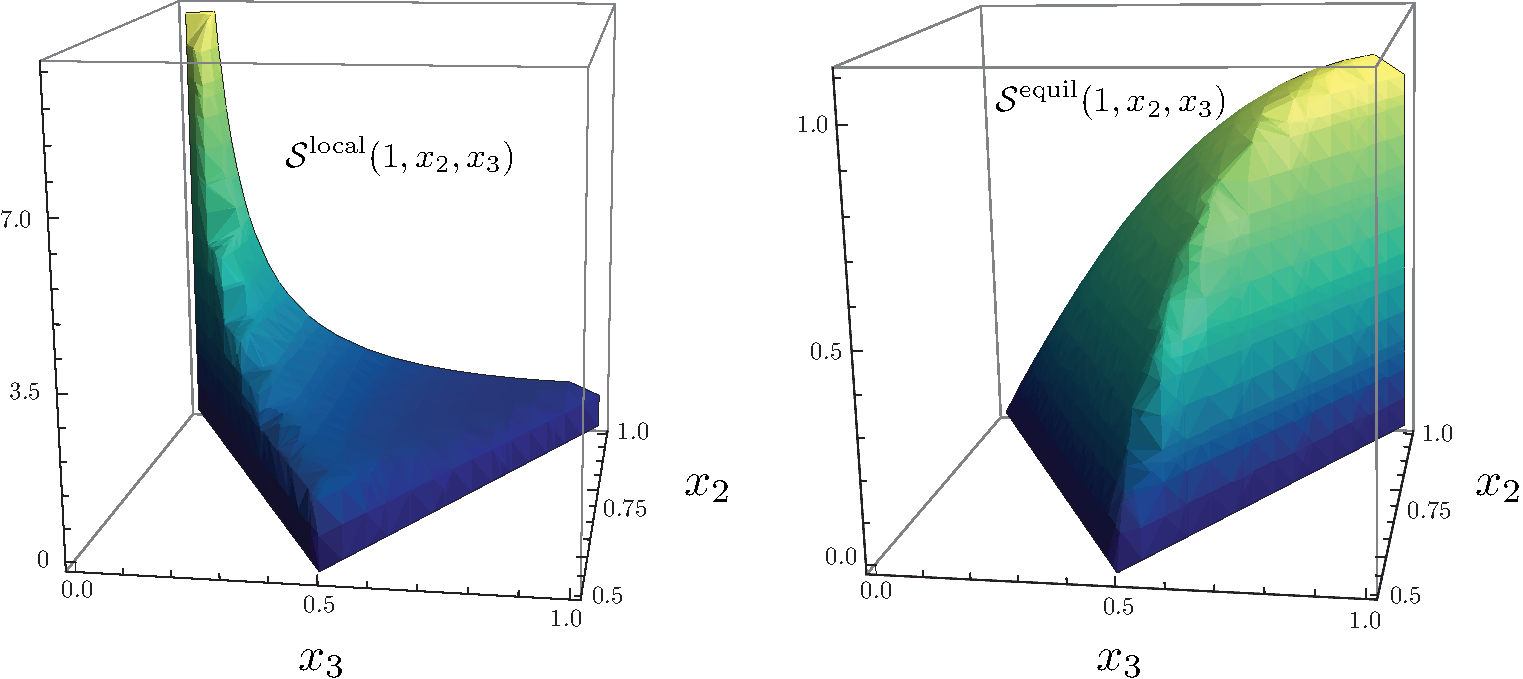
\includegraphics[width=.95\textwidth]{LocalEquil3D}
   \caption{{\it 局所型}および{\it 正三角形型}バイスペクトルの3次元表示．座標 $x_2$ と $x_3$ は，それぞれ再スケールした運動量 $k_2/k_1$ と $k_3/k_1$ である．運動量は $x_3 < x_2< 1$ となるように並べられ，三角不等式 $x_2 + x_3 > 1$ を満たす．}
    \label{fig:localequil}
\end{figure}

\begin{figure}[h!]
    \centering
        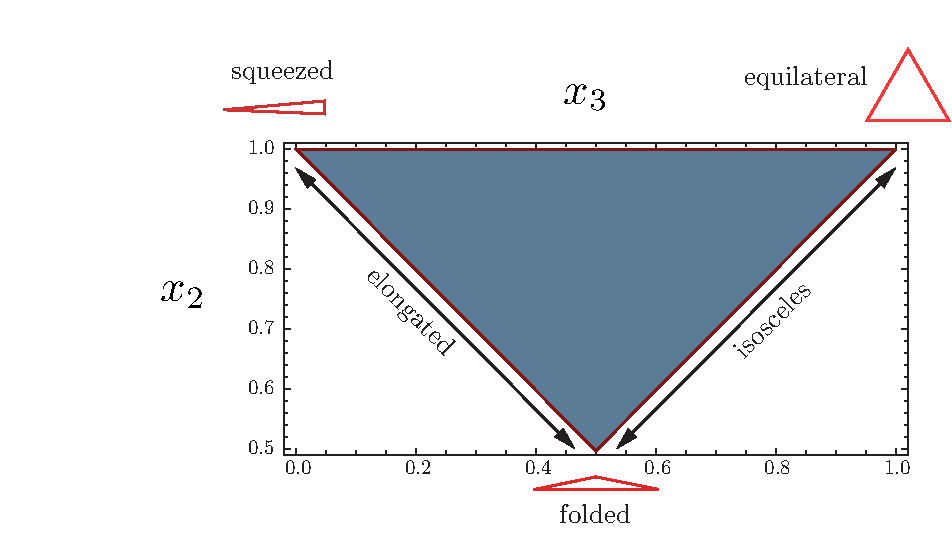
\includegraphics[width=.75\textwidth]{NGShapes}
   \caption{非ガウス性の形状．座標 $x_2$ と $x_3$ は，それぞれ再スケールした運動量 $k_2/k_1$ と $k_3/k_1$ である．運動量は $x_3 < x_2< 1$ となるように並べられ，三角不等式 $x_2 + x_3 > 1$ を満たす．}
    \label{fig:shapes}
\end{figure}

\begin{figure}[h!]
    \centering
        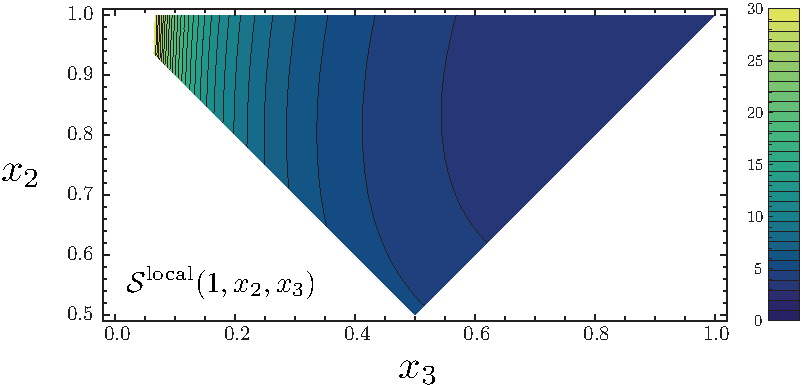
\includegraphics[width=.65\textwidth]{LocalContour}
   \caption{{\it 局所型}バイスペクトルの等高線図．}
    \label{fig:local}
\end{figure}

\begin{figure}[h!]
    \centering
        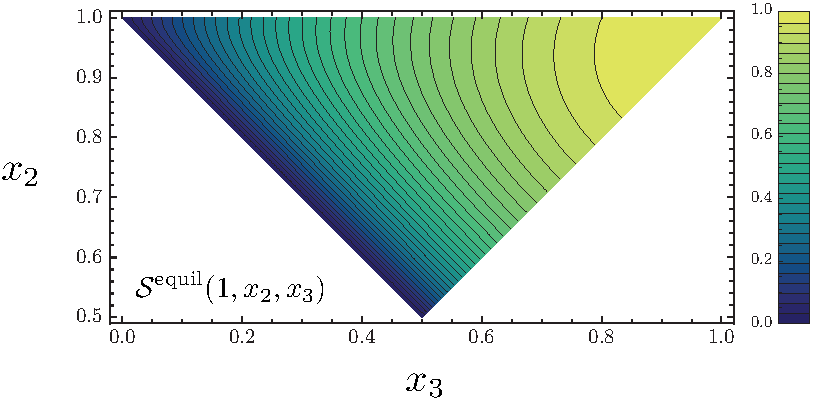
\includegraphics[width=.65\textwidth]{EquilContour}
   \caption{{\it 正三角形型}バイスペクトルの等高線図．}
    \label{fig:equil}
\end{figure}


非ガウス摂動を生成する物理的な動機をもつ模型は，特定の三角形配置でピークをもつ信号を生じることが多い．
重要な三つの特別な場合は次のとおりである：
\begin{enumerate}
\item[i)] {\it スクイーズド三角形}（$k_1 \approx k_2 \gg k_3$）

これは，インフレーション中に複数の軽い場をもつ模型~\cite{BMRmulti, Bernardeau:2002jy, Bernardeau:2002jf, Sasaki:2008uc, Naruko:2008sq, Byrnes:2008wi, Byrnes:2006fr, Langlois:2008vk, Valiviita:2008zb, Assadullahi:2007uw, Valiviita:2006mz, Vernizzi:2006ve, Allen:2005ye}，カーバトン・シナリオ~\cite{Linde:1996gt, Lyth_etal03}，不均一な再加熱~\cite{Dvali:2003em, Kofman:2003nx}，および新エクピロティック模型~\cite{Creminelli:2007aq,Koyama_etal07,Buchbinder_etal07, Lehners:2007wc,Lehners:2008my, Koyama:2007ag, Koyama:2007mg}において支配的なモードである．

\item[ii)] {\it 正三角形}（$k_1 = k_2 = k_3$）

正三角形でピークをもつ信号は，高階微分相互作用と非自明な音速をもつ模型で生じる~\cite{DBI, Chen:2006nt}．

\item[iii)] {\it 折り畳まれた三角形}（$k_1 = 2k_2 = 2 k_3$）

折り畳まれた三角形は，非標準的な初期状態をもつ模型で現れる~\cite{Holman:2007na, Chen:2006nt}．
\end{enumerate}

さらに，中間的な場合として，{\it 引き延ばされた三角形}（$k_1 = k_2 +k_3$）と{\it 二等辺三角形}（$k_1 > k_2 = k_3$）がある．



\subsectionlink{$f_{\rm NL}$：非ガウス性の振幅}

任意の形状関数に対して，一般化された $f_{\rm NL}$ パラメータを定義することで非ガウス性の大きさを測る：
\beq
\label{equ:gfNL}
\fbox{$\displaystyle f_{\rm NL} \equiv \frac{5}{18} \frac{B_\R(k,k,k)}{P_\R(k)^2} $}\, .
\eeq
この定義では，非ガウス性の振幅は正三角形配置で規格化される．

\begin{thm}[$f_{\rm NL}$]
式~(\ref{equ:LocalBi}) を用いて，定義~(\ref{equ:gfNL}) が式~(\ref{equ:local}) による $f_{\rm NL}^{\rm local}$ の定義と整合することを示せ．
  \end{thm}


\sectionlink{理論的予想}

\subsectionlink{単一場のスローロール・インフレーション}

スローロール・インフレーションが成立するには，インフラトン場の相互作用が弱くなければならない．自由場の基底状態の波動関数はガウス型であるため，スローロール・インフレーション中に生成される揺らぎもガウス型と予想される．
Maldacena~\cite{malda}は，スローロール（SR）インフレーションのバイスペクトルを初めて導出した：
\bea
{\cal S}^{\rm SR}(k_1, k_2, k_3) &\propto& ( \varepsilon - 2 \eta) \frac{K_3}{K_{111}} + \varepsilon \left(K_{12} + 8 \frac{K_{22}}{K} \right) \\
&\approx& (4 \varepsilon - 2 \eta) \, {\cal S}^{\rm local}(k_1, k_2, k_3) + \frac{5}{3} \varepsilon \, {\cal S}^{\rm equil}(k_1, k_2, k_3)\, , \label{equ:SSR}
\eea
ここで ${\cal S}^{\rm local}$ と ${\cal S}^{\rm equil}$ は，${\cal S}^{\rm local}(k,k,k) = {\cal S}^{\rm equil}(k,k,k)$ となるように規格化されている．
スローロール・インフレーションのバイスペクトルはスクイーズド三角形でピークをもち，その振幅はスローロール・パラメータによって抑制される~\cite{malda}：
\beq
f_{\rm NL}^{\rm SR} = {\cal O}(\varepsilon, \eta)\, . 
\eeq
スローロール・パラメータはインフラトンの自由場からのずれを特徴づけるので，これは直感にも合っている．

\subsectionlink{Maldacenaの定理}

単一場のインフレーションという仮定のもとで，インフレーションの作用については{\it ほかに何も}仮定せずに，Creminelli と Zaldarriaga~\cite{Creminelli:2004yq}は強力な定理を証明した： %first considered for the special case of slow-roll inflation by Maldacena:
\beq
\label{equ:CZ}
\fbox{$\displaystyle
\lim_{k_3 \to 0} \langle \R_{{\bf k}_1} \R_{{\bf k}_2} \R_{{\bf k}_3} \rangle = (2\pi)^3 \delta({\bf k}_1 + {\bf k}_2 + {\bf k}_3) \, \underline{\underline{(1-n_{\rm s})}} \, P_\R(k_1) P_\R(k_3) $} \, ,
\eeq
ここで
\beq
\langle \R_{{\bf k}_i} \R_{{\bf k}_j} \rangle = (2\pi)^3 \delta({\bf k}_i + {\bf k}_j) P_\R(k_i)\, .
\eeq
式~(\ref{equ:CZ}) は，単一場のインフレーションでは3点関数のスクイーズド極限が ($1-n_{\rm s}$) によって抑制され，完全にスケール不変な摂動では消えることを述べている．
したがって，スクイーズド極限で非ガウス性が検出されれば，単一場のインフレーションを排除できる！
特に，この主張はポテンシャルの形，運動項の形（または音速），および初期真空状態に依存しない．

\vspace{0.5cm}
 \hrule \vspace{0.3cm}
{\bf 証明}：

スクイーズド三角形は，一つの長波長モード $k_{\rm L} = k_3$ と二つの短波長モード $k_{\rm S}=k_1 \approx k_2$ を相関させる：
\beq
\langle \R_{{\bf k}_1} \R_{{\bf k}_2} \R_{{\bf k}_3} \rangle  \approx \langle (\R_{{\bf k}_{\rm S} })^2 \R_{{\bf k}_{\rm L}}\rangle\, .
\eeq
波長の長いモードほど早く凍結する．したがって，二つの短波長モードが凍結する時点で $k_{\rm L}$ はすでに地平線の外で凍結しており，それらに対する背景場として作用する．

なぜ $(\R_{{\bf k}_{\rm S} })^2$ は $\R_{{\bf k}_{\rm L}}$ と相関するのだろうか．
定理によれば，「$\R_{\rm k}$ が厳密にスケール不変なら相関しない」．
証明は実空間で最も簡単になる（Creminelli と Zaldarriaga~\cite{Creminelli:2004yq}参照）：
長波長の曲率摂動 $\R_{{\bf k}_{\rm L}}$ は，あるハッブル領域内の空間座標を再スケールする（あるいは有効なスケール因子を変える）：
\beq
\d s^2 =  - \d t^2 + a(t)^2 e^{2\R} \d {\bf x}^2\, .
\eeq
2点関数 $\langle \R_{{\bf k}_1} \R_{{\bf k}_2} \rangle$ は，地平線の外ですでに凍結している背景揺らぎ $\R_{{\bf k}_{\rm L}}$ の値に依存する．位置空間では，長波長揺らぎ $\R_{\rm L}$ による2点関数の変化は，線形の次数で
\beq
\label{equ:4}
\frac{\partial}{\partial \R_{\rm L}} \langle \R(x) \R(0) \rangle \cdot \R_{\rm L} = x \frac{d}{dx} \langle \R(x) \R(0) \rangle \cdot \R_{\rm L} \, .
\eeq 
3点関数を得るために，Creminelli と Zaldarriaga は式~(\ref{equ:4}) に $\R_{\rm L}$ を掛け，それについて平均を取る．
フーリエ空間に移ると式~(\ref{equ:CZ}) が得られる．\footnote{詳細は Cheung ら~\cite{Cheung:2007sv}を参照．}
証明終．
\vspace{0.2cm}  \hrule
 \vspace{0.5cm}
 

\subsectionlink{大きな非ガウス性をもつ模型}

\subsubsection{高階微分相互作用}


Maldacena は単一場の{\it スローロール}・インフレーションでは非ガウス性が常に小さいことを証明したが，インフレーション中に高階微分項が重要であれば，単一場の模型でも大きな非ガウス性を生じうる（スローロール・インフレーションで仮定する正準的な運動項と高階微分補正の不在を緩める）．
次の作用を考えよう：
\beq
S = \frac{1}{2} \int \d^4 x \sqrt{-g} \left[ R - P(X, \phi)\right]\, , \quad \text{ただし} \quad X \equiv (\partial_\mu \phi)^2\, .
\eeq
ここで $P(X, \phi)$ は運動項 $X=(\partial_\mu \phi)^2$ の任意の関数であり，したがって高階微分相互作用を含みうる．
これらの模型では一般に，揺らぎの伝播の音速が非自明になる：
\beq
c_s^2 \equiv \frac{P_{,X}}{P_{,X} + 2 X P_{,XX}}\, .
\eeq

$\R$ の2次の作用（$P_\R$ を与える）は~\cite{Chen:2006nt}
\beq
S_{(2)} = \int \d^4 x \, \varepsilon \left[ a^3 (\dot \R)^2/ \underline{\underline{c_s^2}} - a (\partial_i \R)^2\right] + {\cal O}(\varepsilon^2)
\eeq
$\R$ の3次の作用（$B_\R$ を与える．付録~\ref{sec:inin}および文献~\cite{Chen:2006nt}参照）は
\beq
\label{equ:s3}
S_{(3)} = \int \d^4 x\, \underline{\underline{\varepsilon^2}} \left[ \dots a^3 (\dot \R)^2 \R/ \underline{\underline{c_s^2}} + \dots a (\partial_i \R)^2 \R + \dots a^3 (\dot \R)^3/ \underline{\underline{c_s^2}} \right] + {\cal O}(\varepsilon^3)
\eeq
3次の作用が2次の作用に比べて余分な $\varepsilon$ の因子によって抑制されていることに注目しよう．
これは，スローロール極限 $P(X, \phi) = X- V(\phi)$，$c_s^2 = 1$ で非ガウス性が小さいことの現れである．
しかしスローロール極限から離れ，音速が小さく $c_s^2 \ll 1$ なる場合には，式~(\ref{equ:s3}) のいくつかの相互作用項が増幅され，非ガウス性が大きくなりうる．
信号は正三角形でピークをもち，
\beq
\label{equ:Lequil:source-duplicate-1}
f_{\rm NL}^{\rm equil} = - \frac{35}{108} \left( \frac{1}{c_s^2} -1 \right) + \frac{5}{81} \left( \frac{1}{c_s^2} - 1 - 2 \Lambda \right)\, ,
\eeq
ここで
\beq
\Lambda \equiv \frac{X^2 P_{,XX} + \frac{2}{3} X^3 P_{,XXX}}{X P_{,X} + 2 X^2 P_{,XX}}\, .
\eeq
任意の $P(X,\phi)$ をもつ作用が整合的な高エネルギー理論に存在するかどうかは，これらの模型にとって重要な課題である．
弦理論における最も興味深いインフレーション模型の一つであるDBIインフレーション~\cite{DBI}（{\bf 第5講}参照）が，まさにこのような構造をもつことは心強い：
\beq
P_{\rm DBI}(X, \phi) = - f^{-1}(\phi) \sqrt{1-2 f(\phi) X} + f^{-1}(\phi) - V(\phi)\, .
\eeq
この場合，式~(\ref{equ:Lequil}) の第2項は恒等的にゼロとなり，次を得る：
\beq
\label{equ:Lequil}
f_{\rm NL}^{\rm DBI} = - \frac{35}{108} \left( \frac{1}{c_s^2} -1 \right) \, .
\eeq
DBIインフレーションの形状関数は
\beq
\label{equ:SDBI}
{\cal S}^{\rm DBI}(k_1,k_2,k_3) \propto \frac{1}{K_{111} K^2} (K_5+ 2 K_{14} - 3 K_{23} +2 K_{113}-8 K_{122})\, .
\eeq

\subsubsection{複数の場}

単一場のスローロール・インフレーションでは，インフラトンの相互作用はインフレーションが生じるという要請によって制約される．
しかし，インフレーション中に複数の場が重要であれば，この制約を回避できる．{\it カーバトン機構}~\cite{Linde:1996gt, Lyth_etal03}や{\it 不均一な再加熱}~\cite{Dvali:2003em, Kofman:2003nx}のような模型は，この点を利用し，インフラトンとは別の第2の場の揺らぎを通して非ガウス揺らぎを生成する．
信号はスクイーズド三角形でピークをもつ．

局所型非ガウス性を生むこれらの機構の詳細については，Bartolo らの総説~\cite{NGreview}を参照されたい．

\subsubsection{非標準的な真空}

インフレーションがBunch--Davies真空ではなく励起状態から始まったなら，残存する非ガウス性が観測可能かもしれない~\cite{Holman:2007na}（ただしインフレーションが最小限の $e$-fold数を大幅に超えて継続した場合には，この効果は指数関数的に希釈される）．
信号は折り畳まれた三角形でピークをもち，その形状関数は
\beq
\label{equ:Sfolded}
{\cal S}^{\rm folded}(k_1,k_2,k_3) \propto \frac{1}{K_{111}} (K_{12} - K_3) + 4 \frac{K_2}{(\tilde k_1 \tilde k_2 \tilde k_3)^2}\, .
\eeq
この効果のより詳しい議論については，Holman と Tolley の論文~\cite{Holman:2007na}を参照されたい．

 
\sectionlink{観測の展望}


原始非ガウス性に対する観測的制約は，興味深い水準に達し始めている．
高精度CMB実験は現在，一部のインフレーション模型~\cite{Linde:1996gt, Lyth_etal03, Dvali:2003em, Kofman:2003nx}と，新エクピロティック模型の大半~\cite{Creminelli:2007aq,Koyama_etal07,Buchbinder_etal07, Lehners:2007wc,Lehners:2008my, Koyama:2007ag, Koyama:2007mg}が信号を予測するパラメータ空間の領域を調べている．

\subsectionlink{宇宙マイクロ波背景放射}

Smith，Senatore，Zaldarriaga~\cite{Smith:2009jr, Senatore:2009gt}による $f_{\rm NL}^{\rm local}$ および $f_{\rm NL}^{\rm equil}$ への最新の制約は
\begin{align}
- 4& \ < \ f_{\rm NL}^{\rm local} \ < \ \ +80 \quad \text{（信頼水準} \ \ 95\% \ \text{）}\, , \\
- 125& \ < \ f_{\rm NL}^{\rm equil} \ < \ \ +435 \quad \text{（信頼水準} \ \ 95\% \ \text{）}\, .
\end{align}
Planck衛星と提案中のCMBPolミッションでは，それぞれ $\sigma(f_{\rm NL}^{\rm local}) \sim 5$ と $\sigma(f_{\rm NL}^{\rm local}) \sim 2$ が得られると予測されている．
実際，$f_{\rm NL} \sim {\cal O}(1)$ の水準では，インフレーションとは無関係な二次効果からの信号が見えると予想される．これらの効果を原始信号と混同しないためには，揺らぎの非線形発展がそれ自身の非ガウス性をどのように誘起するかを詳細に計算する必要がある．
現時点で，これらの効果はまだ完全には計算されていない（ただし，例えば文献~\cite{BMR1, BMR2, Senatore:2008wk}参照）．
多くの場合，その大きさのオーダーだけが見積もられている．観測可能な水準の非ガウス性を誘起するすべての効果を系統的に特徴づけることは，明らかに時宜にかなっている．




\subsectionlink{大規模構造}

非ガウス性は宇宙の大規模構造にも痕跡を残す．
一般に，大規模構造の観測から原始非ガウス性を取り出すことは，非線形揺らぎが原始起源の信号を完全に圧倒する非ガウス性を生むために難しくなる．
しかし最近，原始非ガウス性を探る有望な手段として{\it スケール依存バイアス}の概念が導入された~\cite{Dalal:2007cu, Slosar:2008hx}．
基礎にある密度場を大きなバイアスでたどるトレーサーでは，バイアス・パラメータがスケールと $f_{\rm NL}$ に依存することが示されている~\cite{Dalal:2007cu, Slosar:2008hx}：
\beq
P_{\delta_g}(k) = \left[b+ \Delta b(k, f_{\rm NL}^{\rm local})\right]^2 P_\delta(k)\, .
\eeq
この手法の詳細は本講の範囲を超えるが，例えば文献~\cite{Slosar:2008hx}に述べられている．
この手法をSDSSの高光度赤色銀河（LRG）のサンプルに適用すると，次が得られる~\cite{Slosar:2008hx}：
\beq
- 29 \ < \ f_{\rm NL}^{\rm local} \ < \ + 70 \quad \text{（信頼水準} \ \ 95\% \ \text{）}\, .
\eeq
この上限がCMBから得られた制約に匹敵することに注意しよう．
原始非ガウス性の真に頑健な検証とするにはさらなる研究が必要だが，Slosar らによる予備的な結果~\cite{Slosar:2008hx}は，この手法の原理を実証する心強いものとなっている．

\newpage
\sectionlink{{\sl まとめ}：第4講}

\vskip 10pt


宇宙論的揺らぎの相関に対する非ガウス的寄与の研究は，初期宇宙を探る重要な手段となりつつある~\cite{Komatsu:2009kd}．非ガウス性はインフラトンの相互作用を直接測る量なので，インフレーションのダイナミクスについて多くを教えてくれる可能性がある．

非ガウス揺らぎの基本的な診断量は，3点関数またはバイスペクトルである：
\beq
\langle \R_{{\bf k}_1}  \R_{{\bf k}_2}   \R_{{\bf k}_3} \rangle =(2\pi)^3 \delta({\bf k}_1 + {\bf k}_2 + {\bf k}_3)  B_\R(k_1, k_2, k_3) \, .  \nonumber
\eeq

非ガウス摂動を生成する物理的な動機をもつ模型は，特定の三角形配置でピークをもつ信号を生むことが多い．
三つの特別な場合は次のとおりである：
\begin{enumerate}
\item[i)] {\it スクイーズド三角形}（$k_1 \approx k_2 \gg k_3$）

これは，インフレーション中に複数の軽い場をもつ模型~\cite{BMRmulti, Bernardeau:2002jy, Bernardeau:2002jf, Sasaki:2008uc, Naruko:2008sq, Byrnes:2008wi, Byrnes:2006fr, Langlois:2008vk, Valiviita:2008zb, Assadullahi:2007uw, Valiviita:2006mz, Vernizzi:2006ve, Allen:2005ye}，カーバトン・シナリオ~\cite{Linde:1996gt, Lyth_etal03}，不均一な再加熱~\cite{Dvali:2003em, Kofman:2003nx}，および新エクピロティック模型~\cite{Creminelli:2007aq,Koyama_etal07,Buchbinder_etal07, Lehners:2007wc,Lehners:2008my, Koyama:2007ag, Koyama:2007mg}において支配的なモードである．

\item[ii)] {\it 正三角形}（$k_1 = k_2 = k_3$）

正三角形でピークをもつ信号は，高階微分相互作用をもつ模型で生じる~\cite{DBI}．

\item[iii)] {\it 折り畳まれた三角形}（$k_1 = 2k_2 = 2 k_3$）

折り畳まれた三角形は，非標準的な初期状態をもつ模型で現れる~\cite{Holman:2007na}．
\end{enumerate}

\begin{figure}[h!]
    \centering
        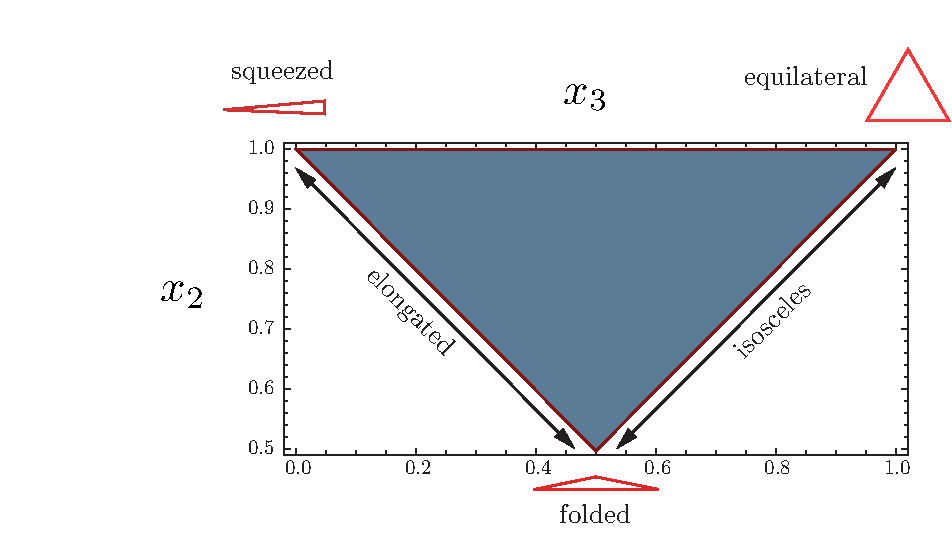
\includegraphics[width=.75\textwidth]{NGShapes}
   \caption{非ガウス性の形状．三角形の形状は，再スケールした運動量 $x_2 = k_2/k_1$，$x_3=k_3/k_1$ によってパラメータ化される．}
    \label{fig:shapes2}
\end{figure}
単一場の整合性関係は
\beq
\lim_{k_3 \to 0} \langle \R_{{\bf k}_1} \R_{{\bf k}_2} \R_{{\bf k}_3} \rangle = (2\pi)^3 \delta({\bf k}_1 + {\bf k}_2 + {\bf k}_3) \, \underline{\underline{(1-n_{\rm s})}} \, P_\R(k_1) P_\R(k_3)  \, . \nonumber
\eeq
これは，単一場のインフレーションのバイスペクトルのスクイーズド極限が，スケール不変性からのずれ $1- n_{\rm s}$ に比例することを述べている．


\sectionlink{{\sl 演習問題}：第4講}

\vskip 10pt
\begin{thmP}[バイスペクトルの図示]\label{ex:bispectra}

局所型および正三角形型のバイスペクトルの図（それぞれ図~\ref{fig:local}と図~\ref{fig:equil}）を再現せよ．
続いて，スローロール・インフレーション，DBI模型，および励起した初期状態をもつ模型のバイスペクトル，すなわち ${\cal S}^{\rm SR}(1,x_2,x_3)$（式~(\ref{equ:SSR})），${\cal S}^{\rm DBI}(1,x_2,x_3)$（式~(\ref{equ:SDBI})），${\cal S}^{\rm folded}(1,x_2,x_3)$（式~(\ref{equ:Sfolded})）を図示せよ．


\end{thmP}
\newpage


\newpage
%\part{Lecture 4: Advanced Topic: Non-Gaussianity}
\part{第5講：弦理論におけるインフレーション}

\vspace{0.5cm}
 \hrule \vspace{0.3cm}
\begin{quote}
{\bf 要旨}

\noindent
この連続講義の最後に，少し高度な話題である弦理論におけるインフレーションを論じる．
Liam McAllisterとの最近の総説論文~\cite{BMReview}に基づき，この主題を教育的に概説する．
本講の中心的な主題は，インフレーションのプランク・スケールの物理に対する感度である．これこそが弦理論でインフレーションを実現する主要な動機であると同時に，中心的な理論的課題でもあると論じる．
弦理論におけるインフレーション・シナリオの二つの事例，ワープしたDブレーン・インフレーションとアクシオン・モノドロミー・インフレーションを通じて，これらの問題を具体的に示す．
最後に，理論面と観測面の両方における今後の進展の可能性を示す．
\end{quote}
\vspace{0.1cm}  \hrule
 \vspace{0.5cm}


\sectionlink{なぜ二つの思弁的な考えを結びつけるのか？}

これまでの講義で，インフレーションが極初期宇宙のダイナミクスの現象論的模型として際立って成功していることを見てきた．しかし，インフレーション的膨張の物理的起源の詳細な理解は，依然として得られていない．
インフレーションと弦理論はいずれも，最高エネルギーでの物理的宇宙を理解しようとする野心的な試みである．
どちらも思弁的な理論であり，実験による確認を待っている．
したがって，なぜ今，弦理論におけるインフレーションという問題に取り組むべきなのかと疑問に思うかもしれない．

本講では，場の量子論と重力の紫外（UV）完備化，すなわちプランク・スケールに近づくエネルギーでの場の内容と相互作用に敏感に依存する，インフレーションの特定の側面を取り上げる．このような問題を最も自然に扱えるのはプランク・スケールの物理の理論であり，弦理論はおそらくその最も発展した候補である．これが，弦理論でインフレーションの物理を理解しようとする動機である．

\S\ref{sec:ST}の弦理論による構成の詳細にはあまり関心がない読者にも，\S\ref{sec:UV}の有効場理論に基づく一般的な議論は参考になるだろう．
 
\sectionlink{インフレーションの紫外物理に対する感度}
\label{sec:UV}


\subsectionlink{有効場理論とインフレーション}
\label{sec:eft}

\begin{figure}[h!]
	\centering
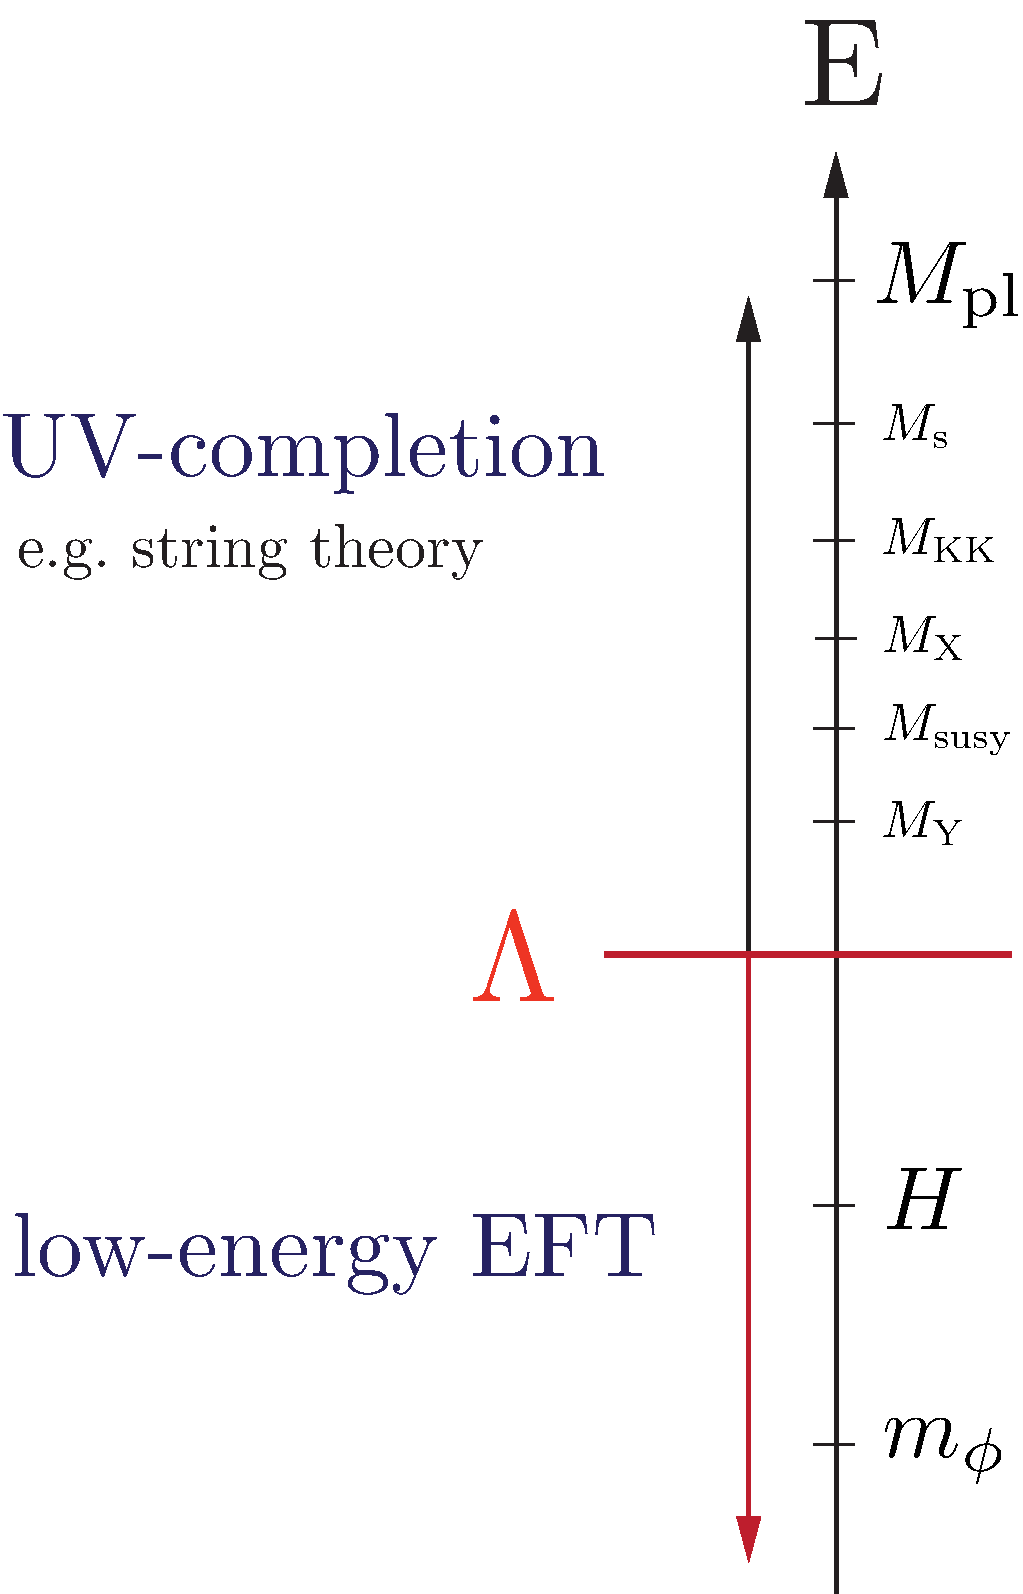
\includegraphics[width=.31\textwidth]{EFT}
%\vspace{-0.5cm}
\caption{インフレーションの有効場理論（EFT）．EFTのカットオフ $\Lambda$ は，低エネルギー理論のスペクトルに含まれない最も軽い粒子の質量によって定義される．カットオフを超える質量をもつ粒子は積分消去され，インフラトンなどの軽い場のラグランジアンに補正を与える．}
\label{fig:EFT}
\end{figure}

一般相対論に結合した場の量子論の現象として見ると，インフレーションは自然とは思われない．特に，インフレーションに適したラグランジアンの集合は，可能なすべてのラグランジアンの集合のごく小さな部分集合である．
さらに，広い範囲の模型で，インフレーションはかなり特殊な初期条件のもとでしか生じない．例えば小場シナリオでは，初期の運動エネルギーがごく小さい配置が必要となる．インフレーションを生むラグランジアンと初期条件の双方の自然さを調べて定量化したいところだが，初期条件の問題は，永遠のインフレーションにおける測度を理解しようとする，活発ではあるものの未完成な研究計画と切り離せないように見える（批判的な評価は\S\ref{sec:conclusion}参照）．
 % \cite{eternal}.
% (However, see {\it e.g.}~\cite{initial} for recent efforts to quantify or to ameliorate the fine-tuning of initial conditions.) 
本講では，インフレーションに適したラグランジアンをもつことがどれほど自然（または不自然）であるかという問題に集中する．

正準的な運動項をもつ単一のインフラトン場では，インフレーションの必要条件をインフラトン・ポテンシャルで表せる（{\bf 第1講}参照）．
インフレーションには，プランク単位で非常に平坦なポテンシャルが必要である：
 \beq
 \epsilon_{\rm v} = \Mp^2 \left(\frac{V_{,\phi}}{V}  \right)^2 \ll 1\, , \qquad \eta_{\rm v} = \frac{\Mp^2}{2} \frac{V_{, \phi \phi}}{V} \ll 1\, .
 \eeq
これから論じるように，この条件はプランク・スケールの物理に敏感である．

$W$--$W$ 散乱のユニタリティが ${\rm TeV}$ スケールの新しい物理を要求するのと同様に，重力子同士の散乱を整合的にするためには，プランク・スケールで何らかの新しい物理が必要であることを思い出そう．新しい自由度が現れなければならないことはわかっているが，プランク・スケールの物理が弦理論のような有限な量子重力理論なのか，それともさらに高いスケールの未知の物理に対する単なる有効理論なのかはわからない．しかし，プランク・スケールの理論の構造は，インフラトン・ポテンシャルの形に有意義な，そして非常に好都合な場合には検証可能な帰結をもたらす．

通常どおり，あるカットオフ $\Lambda$ を超える高スケールの物理の効果は，低エネルギー有効理論の演算子の係数によって効率よく記述される（図~\ref{fig:EFT}参照）．質量 $M \ge \Lambda$ の粒子を積分消去すると，次の形の演算子が生じる：
\begin{equation}
\label{equ:ODelta}
\fbox{$\displaystyle \frac{{\cal{O}}_{\delta}}{M^{\delta-4}} $}\, ,
\end{equation}
ここで $\delta$ は演算子の質量次元を表す．

このような演算子に対する感度は，素粒子物理ではありふれている．例えば，フレーバーを変える過程に対する制限は ${\rm TeV}$ スケールを超える物理を制限し，陽子の寿命の下限からは，陽子崩壊を媒介するGUTスケールの演算子さえ制約できる．
しかし，素粒子物理の考察だけでは，次元 $\delta=6$ を超える演算子や $M\sim M_{\rm GUT}$ を超えるスケールにまで届くことは少ない．（重力を媒介とする超対称性の破れのシナリオは例外の一つである．）同じことを言い換えると，プランク・スケールの過程や非常に高い次元の演算子は，素粒子物理の大部分には無関係であり，低エネルギー現象から分離している．

しかしインフレーションでは，プランク単位でのポテンシャルの平坦性によって，次のような $\delta\le 6$ の{\it プランク・スケールで抑制された}演算子に対する感度が生じる：
\begin{equation}
\label{equ:O6}
\frac{{\cal{O}}_{6}}{M_{\rm pl}^{2}}\, .
\end{equation}
etaパラメータの小ささを論じるには，すなわち理論が少なくとも60~$e$-foldのインフレーション的膨張を可能にすることを保証するには，このような演算子を理解する必要がある．したがって，次元6のプランク・スケールで抑制された演算子に対するこの感度は，すべてのインフレーション模型に共通する．

大場インフレーション模型では，インフラトン作用の紫外物理に対する感度が劇的に高まる．
この重要な種類のインフレーション模型では，ポテンシャルは任意の次元の演算子からなる{\it 無限}級数に敏感になる（\S\ref{sec:lyth}参照）．


\subsectionlink{eta問題}

インフラトン・ポテンシャルを保護する特定の対称性がない場合，ラグランジアンへの寄与として次の一般的な形が
\beq
\fbox{$\displaystyle
\frac{{\cal O}_6}{M_{\rm pl}^2}\, = \, \frac{{\cal O}_4}{M_{\rm pl}^2}\, \phi^2$}\,
\eeq
許される．
次元4の演算子 ${\cal O}_4$ の真空期待値（vev）がインフレーションのエネルギー密度に匹敵し，$\langle{\cal O}_4 \rangle \sim V$ なら，この項はインフラトンの質量に $H$ 程度の補正を，同じことだがetaパラメータに1程度の補正を与え，インフレーション模型の構築に重大な問題をもたらす．
この形の寄与は，プランク・スケールの自由度を積分消去することで生じると考えられる点を，改めて強調しておく．
本節では，このいわゆる{\it eta問題}をまず\S\ref{sec:higgs}で有効場理論において論じ，次に\S\ref{sec:sugraETA}で超重力の例を用いて具体的に示す．

\subsubsection{インフラトン質量の放射不安定性}
\label{sec:higgs}

カットオフ $\Lambda$ をもつ一般的な有効理論（図~\ref{fig:EFT}参照）では，スカラー場の質量は何らかの対称性に保護されていない限りカットオフ・スケールまで走る．
インフレーションの有効理論のカットオフは少なくともハッブル・スケール以上，$\Lambda \ge H$ なので，これは小さなインフラトン質量（$m_\phi \ll H$）が放射補正に対して不安定であることを意味する．
同じことを言えば，etaパラメータは放射補正
\beq
\Delta\eta_{\rm v} = \frac{\Delta m_\phi^2}{3 H^2} \ge 1\, ,
\eeq
を受け，長く続くインフレーションを妨げる．

ここでの困難はヒッグスの階層性問題に似ているが，超対称性だけではインフラトン質量を安定化できない．インフレーションのエネルギーは必然的に超対称性を破り，その結果生じる超多重項内の分裂は $H$ 程度なので，超対称性は小さなインフラトン質量 $m_\phi \ll H$ を保護しない．

\S\ref{sec:LargeField}では，シフト対称性 $\phi\to\phi \, +\, const.$ によってインフラトン・ポテンシャルを保護するという自然な提案を論じる．これはインフラトンを擬南部--ゴールドストーン粒子と同定することに相当する．
このような対称性がなければ，eta問題は，インフレーションを得るためにその作用を微調整する必要があることを示しているように思われる．



\subsubsection{超重力の例}
\label{sec:sugraETA}

eta問題の重要な例は，局所的に超対称な理論，すなわち超重力において生じる~\cite{Copeland:1994vg}．
4次元超重力は超対称な弦コンパクト化の低エネルギー有効理論なので~\cite{PolchinskiOne, Polchinski}，この場合は多くの弦理論インフレーション模型に関係する．

${\cal N} = 1$ 超重力では，スカラー・ポテンシャルの重要な項がF項ポテンシャルである：
\beq
\label{equ:Fterm}
 V_F = e^{K/M_{\rm pl}^2} \left[ K^{\varphi \bar \varphi} D_{\varphi} W \overline{D_{\varphi} W} - \frac{3}{M_{\rm pl}^2} |W|^2 \right]\, ,
\eeq
ここで $K(\varphi, \bar \varphi)$ と $W(\varphi)$ はそれぞれケーラー・ポテンシャルと超ポテンシャルであり，$\varphi$ はインフラトンとする複素スカラー場である．また，$D_{\varphi}W \equiv \partial_{\varphi} W + M_{\rm pl}^{-2}(\partial_{\varphi} K) W$ と定義した．説明を簡単にするため，ほかに軽い自由度がないと仮定したが，ほかの場を含むように式を一般化することは容易である．

ケーラー・ポテンシャルはインフラトンの運動項 $-K_{,\varphi \bar \varphi} \, \partial \varphi \partial \bar \varphi$ を決め，超ポテンシャルは相互作用を決める．
インフラトン質量を導くため，ある原点のまわりで $K$ を展開する．一般性を失わずにこの原点を $\varphi \equiv 0$ と表すと，$K(\varphi, \bar \varphi) = K_0 + \left. K_{,\varphi \bar \varphi}\right|_0 \, \varphi \bar \varphi + \cdots\ $ である．するとインフレーションのラグランジアンは
\begin{eqnarray}
{\cal L} &\approx& - K_{,\varphi \bar \varphi}\, \partial \varphi  \partial \bar \varphi -  V_0 \Bigl(1+ \left. K_{,\varphi \bar \varphi}\right|_0 \frac{\varphi \bar \varphi}{M_{\rm pl}^2} + \dots \Bigr) \\
&\equiv& -  \partial \phi \partial \bar\phi - V_0 \Bigl(1+  \frac{\phi \bar \phi}{M_{\rm pl}^2} \Bigr) + \dots\, , \label{equ:mid}
\end{eqnarray}
ここで，正準的なインフラトン場 $\phi\bar\phi \approx  \left. K_{\varphi \bar \varphi}\right|_0 \varphi \bar \varphi$ と $V_0 \equiv \left. V_F\right|_{\varphi =0}$ を定義した．
式~(\ref{equ:Fterm}) の $e^{K/M_{\rm pl}^2}$ の展開に由来するポテンシャルへの主要な補正を残してある．これはF項シナリオにおける普遍的な補正と呼んでよいだろう．省略した項の一部は残した項と同じ程度になりうるが，それらは式~(\ref{equ:Fterm}) の
\beq\left[ K^{\varphi \bar \varphi} D_{\varphi} W \overline{D_{\varphi} W} - \frac{3}{M_{\rm pl}^2} |W|^2 \right]
\label{equ:md}
\eeq を展開することで生じ，ケーラー・ポテンシャルと超ポテンシャルの模型依存の構造に明らかに依存する．

結果は式~(\ref{equ:O6}) の形をもち，
\beq
{\cal O}_6 =   V_0\, \phi\bar\phi
\eeq
であることから，etaパラメータへの大きな模型非依存の寄与
\beq
\label{equ:sugraETA}
\Delta \eta_{\rm v} = 1\, ,
\eeq
が生じる．これに加えて，通常は同じ程度の模型依存の寄与がある．したがって，F項ポテンシャルによって駆動されるインフレーション・シナリオでは，etaは一般に1程度になることが明らかである．

超対称なラグランジアンに基づく模型で，それでもインフレーションが起こるのはどのような場合だろうか．明らかな可能性の一つは，etaへの模型依存の寄与~(\ref{equ:md}) が模型非依存の寄与~(\ref{equ:mid}) をほぼ相殺し，インフラトン質量の小ささが微調整の結果として生じることである．\S\ref{sec:warped}の事例研究では，etaへのすべての関連する寄与の構造を計算でき，このような微調整の議論を意味のある形で進められる具体例を示す．

すべての補正が小さく $\Delta \eta_{\rm v} \ll 1$ となることを保証してeta問題を{\it 取り除く}機構を示せれば，明らかにはるかに満足のいくことであろう．そのためには，F項ポテンシャルが無視できるか，またはインフラトンがF項ポテンシャルに現れないことが必要である．第1の場合はあまり生じない．現在理解されている弦理論のコンパクトな次元の安定化模型では，F項ポテンシャルが重要な役割を果たすためである~\cite{KKLT}．
しかし\S\ref{sec:LargeField}では，インフラトンがアクシオンであり，摂動論のどの次数でもケーラー・ポテンシャルにもF項ポテンシャルにも現れないシナリオを提示する．
これにより，上で述べた特定の形のeta問題を回避できる．


\subsectionlink{Lyth限界}
\label{sec:lyth}

{\bf 第2講}で，Lyth限界を導いた~\cite{Lyth:1996im}：
\beq
\frac{\Delta \phi}{M_{\rm pl}} \simeq {\cal O}(1) \left(\frac{r}{0.01}\right)^{1/2}\, ,
\eeq
ここで $r$ はCMBスケールにおけるテンソル・スカラー比の値である．
%, $r_\star \equiv r(N_{\rm cmb})$.
したがって $r >0.01$ をもつどの模型でも，超プランク的な範囲 $\Delta \phi > M_{\rm pl}$ にわたって $\epsilon_{\rm v}, |\eta_{\rm v}| \ll 1$ が成り立つことを保証しなければならない．
この結果は，{\it 大場インフレーション}に対して二つの必要条件を意味する：
\begin{enumerate}
\item[i)] 明らかな要請は，大きな場の変位範囲が{\it 運動学的に}許されること，すなわちスカラー場の場の空間の直径が（正準的な単位で）$> M_{\rm pl}$ となることである．
典型的な弦コンパクト化では，多くの場にこのような大きな変位が許されないため，これは非自明である．
\item[ii)] インフラトン・ポテンシャルの平坦性を，超プランク的な場の範囲にわたって{\it 力学的に}制御する必要がある．
この課題を，\S\ref{sec:EFT}では有効場理論において，\S\ref{sec:LargeField}では弦理論において論じる．
\end{enumerate}

\subsectionlink{超プランク的な場と平坦なポテンシャル}
\label{sec:EFT}

まず，ウィルソン的な有効場理論の枠組みで，超プランク的な場の変位を考えよう．

\subsubsection{シフト対称性がない場合}

特別な対称性がない場合，大場インフレーションのポテンシャルは，プランク・スケールで抑制された演算子の無限級数に敏感になる．
これらの項の物理的解釈は次のとおりである．インフラトンの期待値が変化すると，それに結合するほかの場 $\chi$ は，質量，自己結合などの変化を受ける．
特に，インフラトンに少なくとも重力程度の強さで結合する場は，インフラトンが超プランク的な変位をするときに大きな変化を受ける．
これらの $\chi$ の質量と結合の変化は，今度はインフラトン・ポテンシャルの変化に跳ね返り，インフレーションに必要な繊細な平坦性を損なうおそれがある．
これは軽い自由度だけでなく，プランク・スケールに近い質量をもつ場にも当てはまることに注意しよう．プランク・スケールの自由度を積分消去すると，一般に（すなわち結合が1程度の場合），プランク・スケールで抑制された演算子が有効作用に導入される．素粒子物理のほとんどすべての問題ではこのような演算子は無視できるが，インフレーションでは重要な役割を果たす．

現れる具体的な演算子は，いつもどおり低エネルギー作用の対称性によって決まる．例えば，インフラトンに対称性 $\phi \to - \phi$ だけを課すと，次の有効作用が得られる：
\beq
\fbox{$\displaystyle
{\cal L}_{\rm eff}(\phi) = -\frac{1}{2}(\partial \phi)^2 - \frac{1}{2} m^2 \phi^2 - \frac{1}{4} \lambda \phi^4 - \sum_{p=1}^\infty \left[ \lambda_p \phi^4  + \nu_p (\partial \phi)^2    \right] \left( \frac{\phi}{M_{\rm pl}} \right)^{2p}+ \cdots $}\ .
\eeq
紫外理論がさらなる対称性をもたない限り，係数 $\lambda_p$ と $\nu_p$ は1程度と予想される．
したがって，十分に強力な対称性で保護されていない方向に $\phi$ が $M_{\rm pl}$ 程度の距離を移動すると，そのたびに有効ラグランジアンは高次元演算子の無限級数から大きな補正を受ける．
当然，インフレーションを起こすには，ポテンシャルが超プランク的な範囲にわたってほぼ平坦でなければならない．これが偶然や微調整によって実現されるには，無限個の係数が協調して調整される必要がある．これは「関数的微調整」と呼ばれてきた（一つの質量パラメータの調整だけを必要とするeta問題と比較されたい）．


\subsubsection{シフト対称性がある場合}

この無限級数の補正を制御する合理的な方法がある．インフラトン・ポテンシャルの構造を損なうような仕方でインフラトンがほかの場と結合することを禁じる近似対称性を用いればよい．そのようなシフト対称性
\begin{equation}
\phi \to \phi + const. \, ,
\end{equation}
は，インフラトン・ポテンシャルを自然に保護する．

シフト対称性がある場合，小さな係数 $\lambda_p$ をもつカオス的インフレーションの作用~\cite{Linde:1983gd}
 \beq
 {\cal L}_{\rm eff}(\phi) =- \frac{1}{2} (\partial \phi)^2 - \lambda_p\, \phi^p\, ,
 \eeq
は「技術的に自然」である． % in the sense of 't~Hooft.
しかし，この対称性がプランク・スケールの自由度との結合からさえインフラトンを保護することを要求するため，プランク・スケールの理論でもその対称性が近似的に保たれていることが不可欠である．言い換えれば，低エネルギー有効作用に提案された対称性には紫外完備化が存在しなければならない．したがって，大場インフレーションは，プランク・スケールでの近似対称性の情報にアクセスできる理論の中で定式化すべきである．一般の有効場理論では，仮定した低エネルギー対称性の紫外完備化が喫緊の問題となることはまれであると付記しておこう．現在の状況が異なるのは，妥当な有効作用がすべて実際に弦理論の低エネルギー極限として生じうるかどうかを，われわれが{\it 知らない}ためである．実際，多くの有効理論には弦理論における紫外完備化が存在しないという予想が提案されている~\cite{Vafa:2005ui,Ooguri:2006in, Adams:2006sv}．したがって，プランク・スケールの物理に提案する対称性が，実際に弦理論で実現できるかを確認することが重要である．

したがって，検出可能な重力波を伴うインフレーション模型を構築するためには，弦理論の完全な理論で近似的に保たれるシフト対称性に保護されたポテンシャルと，大きな運動学的範囲の両方をもつ配置を，弦理論の中で見いだすことが目標となる．




\sectionlink{弦理論におけるインフレーション}
\label{sec:ST}

\subsectionlink{弦コンパクト化からインフラトン作用へ}

\begin{figure}[h!]
	\centering
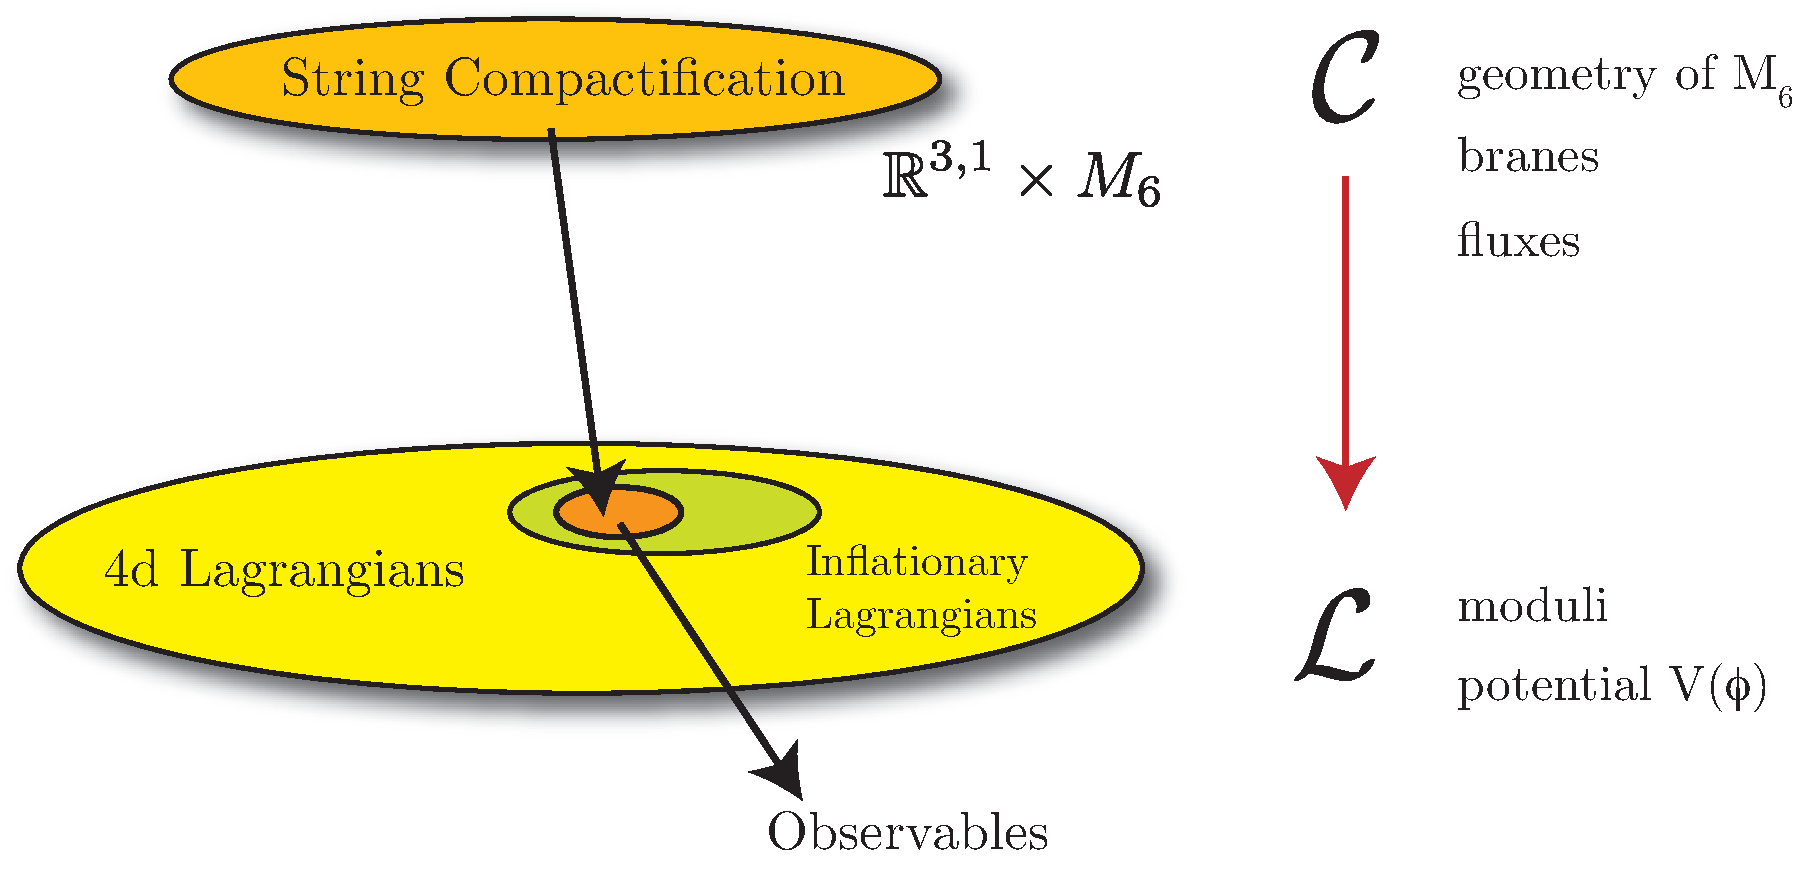
\includegraphics[width=.8\textwidth]{Philosophy}
%\vspace{-0.5cm}
\caption{10次元のコンパクト化データから4次元の作用へ．}
\label{fig:10}
\end{figure}

\subsubsection{弦コンパクト化の構成要素}

弦の量子論は4次元を超える時空次元で自然に定義され，余分な空間次元をコンパクト化すると4次元の物理が現れることはよく知られている．具体的には，臨界10次元IIB型弦理論を6次元カラビ--ヤウ空間上にコンパクト化する場合に焦点を絞る．\footnote{この用語に馴染みのない読者には，文献~\cite{Hertzberg:2007ke}にある弦理論用語から普通の英語への辞書が役立つだろう．}
% (to be precise, our compactifications will only be conformal to spaces that are well-approximated by orientifolds of Calabi-Yau manifolds, but we will not need this fine point.)

この種類に属する膨大な数の異なるコンパクト化は，位相，幾何，および量子化されたフラックスや巻き付いたDブレーンなどの離散的データによって区別される．
弦理論の模型構築における中心的な課題は，10次元の源が4次元有効理論をどのように決定するかを詳細に理解することである（図~\ref{fig:10}参照）．
10次元のコンパクト化データを ${\cal C}$ と表すと，この手順は模式的に
\beq
\label{equ:S10S4}
{\cal S}_{10}[{\cal C}] \quad \to \quad  {\cal S}_4\, .
\eeq
異なるコンパクト化データ ${\cal C}$ からは，場の内容，運動項，スカラー・ポテンシャル，対称性の性質がさまざまに異なる多数の4次元有効理論 ${\cal S}_4$ が生じる（これが弦理論の解の{\it ランドスケープ}である）．
可能なデータ ${\cal C}$ の空間と式~(\ref{equ:S10S4}) の写像の性質を理解することで，興味深い4次元の物理を生むコンパクト化を特定し，さらには分類できるかもしれない．


\begin{figure}[h!]
	\centering

\includegraphics[width=.4\textwidth]{FluxCompactification}
%\vspace{-0.5cm}
\caption{フラックス・コンパクト化の構成要素：フラックスと巻き付いたブレーン．}
\label{fig:flux}
\end{figure}

\subsubsection{インフラトンの有効作用}

われわれの目的にとって，有効理論の最も重要な自由度は4次元スカラー場である．{\it モジュライ}として知られるスカラー場は，コンパクト化多様体の変形から生じ，ここで考えるカラビ--ヤウ空間では通常数百個に上る．また，存在するDブレーンの位置，向き，およびゲージ場の配置からも生じる．与えられたコンパクト化データから，モジュライの運動項とスカラー・ポテンシャルを計算できる．そして，モジュライの期待値が4次元有効理論のパラメータを決める．Dブレーンや量子化されたフラックスのような一般的な10次元のエネルギー運動量源があると，コンパクト化を変形するにはエネルギーが必要となり，多くの（ただし必ずしもすべてではない）モジュライ場が質量を獲得する~\cite{Douglas:2006es}．

${\cal S}_4$ に現れるスカラー場を，質量がハッブル・スケールより小さい軽い場 $\phi,\psi$（$m_\phi, m_\psi \ll H$）と，質量がハッブル・スケールよりはるかに大きい重い場 $\chi$（$m_\chi \gg H$）に分けると便利である．ここで，軽い場の一つを $\phi$ と記し，インフラトン候補と同定する．

適切なインフレーションが生じうるかを理解するには，重い場も軽い場も含め，すべてのスカラー場を理解しなければならない．まず，十分に重いモジュライ場はインフレーション中に事実上凍結しているため，それらを積分消去し，軽い場だけの有効作用を得るべきである：
\beq
{\cal S}_4(\phi, \psi, \chi) \quad \to \quad {\cal S}_{4, \rm eff}(\phi,\psi)\, .
\eeq
これらの重いモードの積分消去は一般に，インフラトン候補のポテンシャルに寄与を誘起する．すなわち，{\it モジュライ安定化はeta問題に寄与する}．
これは，\S\ref{sec:eft}の有効場理論の議論で高次元演算子による補正が現れたことと，完全に類似している．

次に，インフラトン以外のスカラー場もインフレーション中に軽ければ，通常それらはダイナミクスに重要な影響を及ぼすため，質量 $m_\psi \ll H$ をもつすべての場 $\psi$ の発展を調べるべきである．さらに，結果として生じる多場インフレーションのダイナミクスが適切であっても，軽い自由度は後期宇宙論で問題を引き起こしうる．軽いスカラー場はインフレーション中にエネルギーを吸収し，インフレーション後も存在し続ければ，ビッグバン元素合成の最中またはその後にこのエネルギーを放出して，軽元素存在量についての成功した予測を損なう可能性がある．また，軽いモジュライは重力程度の強さの第5の力を媒介するため，現在の宇宙でも問題になる．これらの後期の問題を避けるには，$m_\psi \gg 30 ~\rm{TeV}$ を保証すれば十分である．この場合，モジュライはビッグバン元素合成の前に崩壊する．簡単化のため，インフラトン以外のすべての場が $m \gg H$ を満たすと仮定することもあるが，これは物理的に必須ではない．インフレーション中の有効理論がただ一つの自由度だけをもつようにするための仮定にすぎない．



\subsectionlink{{\sl 事例研究：}ワープしたDブレーン・インフレーション}
\label{sec:warped}

弦理論のインフレーション模型では，インフラトン・ポテンシャルに寄与する演算子を列挙でき，原理的にはその係数さえも与えられたコンパクト化データによって計算できる．
これらの問題を具体的に示すには，特定の模型を詳しく調べると有用である．
そこで以下では，比較的よく理解されている小場インフレーション模型である，{\it{ワープしたDブレーン・インフレーション}}を事例として取り上げる．

\subsubsection{ワープしたスロート幾何におけるD3ブレーン}

このシナリオでは，安定化されたコンパクト空間のワープしたスロート領域内でのD3ブレーンの運動がインフレーションを駆動する~\cite{KKLMMT}．
4次元のローレンツ（またはド・ジッター）不変性を保つため，D3ブレーンはわれわれの4次元時空を満たし，余剰次元内では点状である（図~\ref{fig:throat}参照）．
\begin{figure}[h!]
	\centering
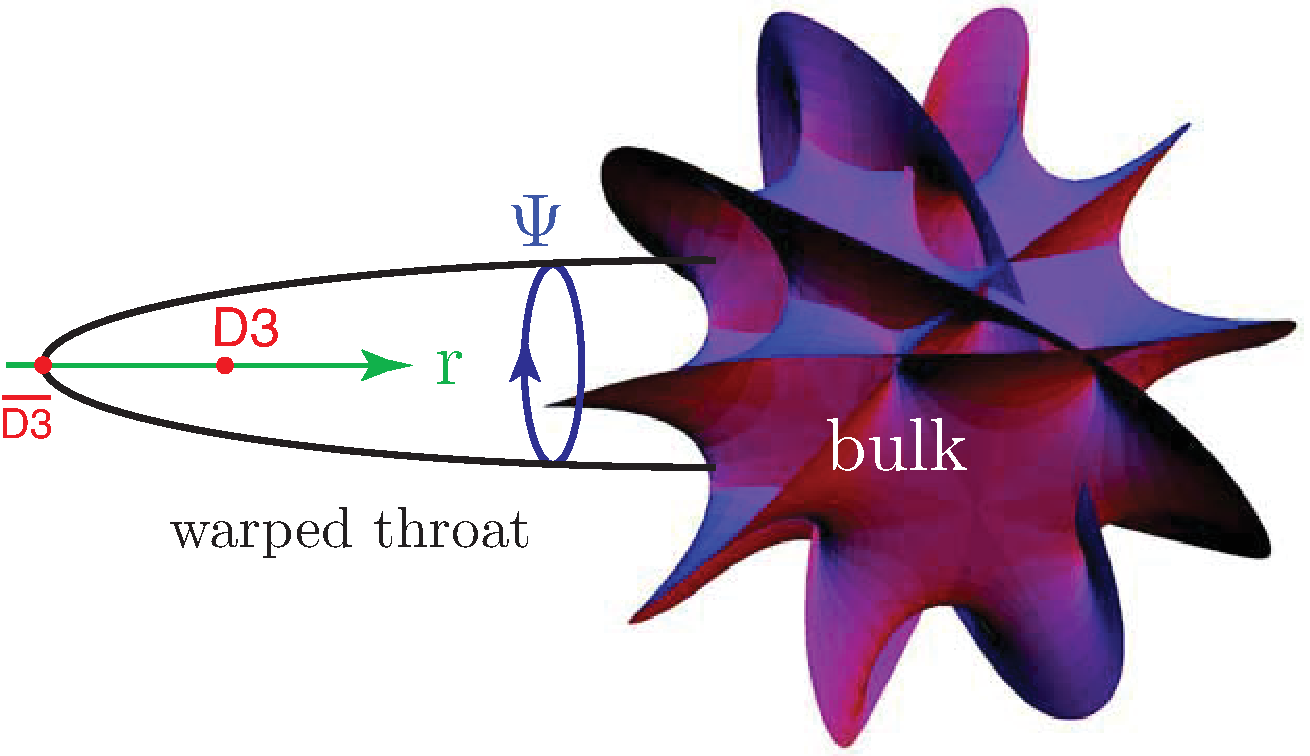
\includegraphics[width=.65\textwidth]{KKLMMT}
%\vspace{-0.5cm}
\caption{ワープしたスロート幾何におけるD3ブレーン・インフレーション．D3ブレーンは4次元時空を満たすため，余剰次元内では点状である．円は角度座標 $\Psi$ をもつ底多様体 $X_5$ を表す．ブレーンは動径方向 $r$ に運動する．$r_{\rm UV}$ でスロートはコンパクトなカラビ--ヤウ空間につながる．反D3ブレーンは，スロートの先端 $r_{\rm IR}$ でエネルギーを最小にする．}
\label{fig:throat}
\end{figure}
コンパクト化の大域的構造は，4次元時空（計量 $g_{\mu \nu}$）とカラビ--ヤウ空間に共形な空間とのワープ積であると仮定する：
\beq
\label{equ:metric}
\d s^2 = e^{2A(y)} g_{\mu \nu} \d x^\mu \d x^\nu + e^{-2A(y)} g_{mn} \d y^m \d y^n \, ,
\eeq
ここで $g_{mn}$ はカラビ--ヤウ計量であり，ある領域では5次元アインシュタイン多様体 $X_5$ 上の錐として近似できる：
\beq
g_{mn} \d y^m \d y^n = \d r^2 +r^2 \d s_{X_5}^2\, .
\eeq
このようなスロート領域の典型例がKlebanov--Strassler（KS）幾何である~\cite{KS}．この場合，$X_5$ は $\Bigl(SU(2)\times SU(2)\Bigr)/U(1)$ の剰余空間 $T^{1,1}$ であり，スロートの先端 $r=0$ に生じるはずの錐特異点は，適切なフラックスの存在によって滑らかになる．
したがって，スロートの先端は有限の動径座標 $r_{\rm IR}$ に位置し，一方 $r=r_{\rm UV}$ でスロートはワープしていないバルク幾何に接続される．
関連する領域 $r_{\rm IR} \ll r < r_{\rm UV}$ では，ワープ因子は次のように書ける~\cite{KT}：
\beq
\label{equ:warp}
e^{-4A(r)} = \frac{R^4}{r^4} \ln \frac{r}{r_{\rm IR}}\, , \qquad R^4 \equiv \frac{81}{8} (g_s M \alpha')^2\, ,
\eeq
ここで
\beq
\ln \frac{r_{\rm UV}}{r_{\rm IR}} \approx \frac{2\pi K}{3 g_s M}\, .
\eeq
ここで $M$ と $K$ はフラックス背景を指定する整数である~\cite{KS,GKP}．
% and $g_s < 1$ is the string coupling.

フラックスを源とするワープは現代のコンパクト化で一般的であり，このようなコンパクト化のモジュライの安定化の理解も大きく進んでいる~\cite{Douglas:2006es}．
したがって，現在の知識に照らせば，KSスロートを含む安定化されたコンパクト化を仮定することは妥当と思われる．


\subsubsection{場の変位範囲の限界}

インフレーション・ポテンシャルの形という複雑な問題に取り組む前に，これらの模型がそもそも大きな振幅の重力波を生みうるかを考えよう．
この問題は純粋に幾何学的な形で表すことができ，インフレーションのダイナミクスの詳細には依存しないことがわかる~\cite{Baumann:2006cd}．
Lyth限界から，大きな重力波信号には超プランク的な場の変位が必要であることがわかっている．そこで最小限の要請として，ワープしたDブレーン・インフレーションで超プランク的な場の値に到達できるかを問う．

インフラトンの運動項はプローブD3ブレーンのDirac--Born--Infeld（DBI）作用によって決まり，正準的なインフラトン場は動径座標の定数倍と同定される：$\phi^2 \equiv T_3 r^2$．ここで $T_3 \equiv \left[(2\pi)^3 g_s \alpha'^2 \right]^{-1}$ はD3ブレーンの張力であり，$g_s$ は弦結合，$2\pi\alpha'$ は弦の張力の逆数である．
スロートの長さ $\Delta r = r_{\rm UV} - r_{\rm IR} \approx r_{\rm UV}$ は，インフラトン場の変位の上限を与える：
\beq
\Delta \phi^2 \ < \ T_3\, r_{\rm UV}^2\, .
\eeq
素朴には，スロートの長さを増やすだけで，これをいくらでも大きくできるように思える．しかしそうするとコンパクト空間の体積が変わり，インフラトンの変位を測る単位である4次元プランク質量にも影響する．
この効果を考慮するため，次元縮約によって4次元プランク質量 $\Mp$ と10次元重力結合 $\kappa_{10}^2 = \frac{1}{2} (2\pi)^7 g_s^2 (\alpha')^4$ が次のように関係づけられることに注目する：
\beq
\Mp^2 = \frac{V_6}{\kappa_{10}^2}\, ,
\eeq
ここで $V_6 \equiv \int \d^6 y \sqrt{g} e^{2A(y)}$ は内部空間の（ワープした）体積である．$\Delta \phi/\Mp$ の上限を求めたいので，スロート領域の体積を用いて $V_6$ に下限を与える（バルク体積の見積もりも含めれば，結論はさらに強まるだけである）：
\beq
V_6 \ > \ (V_6)_{\rm throat} = {\rm Vol}(X_5) \int_0^{r_{\rm UV}} \d r \, r^5 e^{2A(r)} = 2\pi^4 g_s N (\alpha')^2 r_{\rm UV}^2\, ,
\eeq
ここで $N \equiv M K$ は背景フラックスの大きさを表す．超重力近似を制御するには（また背景に十分なワープを実現するには），$N \gg 1$ が必要である．
以上を組み合わせると，次を得る~\cite{Baumann:2006cd}：
\beq
\fbox{$\displaystyle
\frac{\Delta \phi}{\Mp} \ < \ \frac{2}{\sqrt{N}} $} \, .
\eeq
$N \gg 1$ なので，インフラトンの変位は常にプランク・スケール未満，$\Delta \phi \ll \Mp$ であり，重力波の振幅は必然的に小さい．
この議論が純粋に幾何学的で，次に論じるインフレーション・ポテンシャルの複雑な詳細には依存しなかったことを，再び強調しておく．

\subsubsection{D3ブレーンのポテンシャル}
\label{sec:gravity}

インフレーションは，D3ブレーンがスロート領域の動径方向に内側へ，自然にスロートの先端に位置する反D3ブレーンに向かって移動するにつれて進行する．
%The inflaton kinetic term is determined by the Dirac-Born-Infeld (DBI) action for a probe D3-brane, and leads to an identification of the canonical inflaton field with a multiple of the radial coordinate, $\phi^2 \equiv T_3 r^2$. Here, $T_3 \equiv \left[(2\pi)^3 g_s \alpha'^2 \right]^{-1}$ is the D3-brane tension, with $g_s$ the string coupling and $2\pi\alpha'$ the inverse string tension.  
接近する対の間に張られた開弦がタキオン的になって凝縮し，ブレーンが消滅すると，インフレーションが終わる．


この単純化した描像では，インフレーションはブレーン・反ブレーン対の極めて弱い（ワープによって抑制された）クーロン相互作用により駆動される~\cite{KKLMMT}．しかし実際はもっと複雑である．モジュライ安定化がインフラトン・ポテンシャルに新たな項を導入し，それらが通常クーロン項を圧倒して，より複雑なダイナミクスを駆動するためである~\cite{KKLMMT,Baumann:2006th, Baumann:2007np, Baumann:2007ah, Krause:2007jk, Baumann:2008kq}．この構図は，有効場理論の議論から予想したとおりである．モジュライ場を積分消去すると，ポテンシャルに重要な補正が誘起されると期待される．

\vskip 6pt
モジュライ安定化によって誘起される重要な補正は，\S\ref{sec:sugraETA}の超重力のF項ポテンシャルから生じるインフラトン質量項である．F項ポテンシャル，すなわちモジュライを含む超ポテンシャル項によって安定化された真空では，質量項 $H^2_0 \phi^2 = \frac{1}{3} V_0(\phi_\star) \frac{\phi^2}{M_{\rm pl}^2}$ が得られる~\cite{KKLMMT}．
ここで $\phi_\star$ はインフラトン場の任意の基準値であり，パラメータ $H_0$ を現在のハッブル定数と混同してはならない．

しかし，コンパクト化における超対称性を破る追加効果など，ほかのさまざまな起源からもポテンシャルへの寄与が予想される~\cite{Baumann:2008kq}．クーロン相互作用 $V_{0}(\phi)$ と質量項 $H_0^2 \phi^2$ 以外のポテンシャルへのすべての寄与をまとめて $\Delta V(\phi)$ と定義しよう．すると，全ポテンシャルとそれに伴うetaパラメータへの寄与は次のように書ける：
\begin{eqnarray}
\label{equ:Vphi}
V(\phi) &=& V_{0}(\phi) \ \, + \ H^2_0 \phi^2 \ + \ \Delta V(\phi) \\
\eta_{\rm v}(\phi) &=& \quad \eta_0 \quad +  \quad\frac{2}{3} \ \ \ \ + \  \Delta \eta_{\rm v}(\phi) \quad = \quad  ?
\end{eqnarray}
ここで，クーロン相互作用は非常に弱いため $\eta_0\ll 1$ である．
（より一般には，$V(\phi)$ のうち $\eta$ への寄与が無視できるすべての項を $V_0(\phi)$ と{\it 定義}できる．これにはブレーン・反ブレーン間のクーロン相互作用だけでなく，例えば宇宙定数へのバルクからの寄与など，ほぼ一定のエネルギーのほかの起源も含められる．）

明らかに，$\eta_{\rm v}$ が小さくなりうるのは，$\Delta V$ が式~(\ref{equ:Vphi}) の質量項を相殺できる場合に限られる．したがって，$\Delta V$ への関連するすべての寄与を列挙し，どのような状況で近似的な相殺が起こりうるかを理解しなければならない．ほかの寄与を知らないまま $\Delta V$ への一部の寄与だけを特定しても不十分であることに注意しよう．

ワープしたDブレーン・インフレーションが理論的に大きな注目を集めてきた理由の一つは，計算可能性が高いことである．ごく一般に，曲率が小さく弦結合が弱い，明示的で安定化されたコンパクト化の全データが得られれば，注意深く次元縮約を行うことにより，原理的にはDブレーン・インフラトンのポテンシャルを任意の精度まで計算できる．一般のコンパクトなカラビ--ヤウ空間でこれが現在不可能なのは，二つの理由による．一般のカラビ--ヤウ空間について計量データがほとんど得られていないことと，モジュライ安定化が完全に明示された例がまれなことである．

しかし，十分に長いスロートは{\it 非コンパクトな}スロート幾何（すなわち無限に長いスロート）でよく近似でき，そのカラビ--ヤウ計量はしばしば求められる．重要な例が，完全に明示的で至る所滑らかなKlebanov--Strassler解~\cite{KS}である．完全な計量データがあると，少なくともまだ安定化されていないコンパクト化の段階では，プローブDブレーンのダイナミクスの研究が大幅に容易になる．
さらにこれから，モジュライ安定化とスロートの有限の長さの効果を系統的に取り込む方法を説明する．この方法では，D3ブレーンが運動するスロートを記述する超重力解の摂動を調べる．具体的にはKSスロートを例として扱うが，方法自体ははるかに一般的である．
この扱いによって，式~(\ref{equ:Vphi}) の補正項 $\Delta V$ を明示的に表し，モジュライ安定化がある場合のインフレーションの特徴を取り出せる．

\subsubsection{超重力による解析の概要}

以下では，ワープしたD3ブレーン・インフレーションのインフラトン・ポテンシャルの計算を説明する．
これは完全なポテンシャルを理解するうえでの課題の雰囲気を示すためだけのものである．詳細については文献~\cite{KKLMMT, Baumann:2006th, Baumann:2007ah, Baumann:2008kq, Baumann:2007np}を参照されたい．

IIB型弦理論は，ディラトン，$p$形式フラックス，ワープ因子，計量摂動などの名で呼ばれる十数個の場を含む．原理的には，これらすべての場がインフラトン自由度に結合する可能性を考慮し，望む精度でインフラトン・ポテンシャルを計算する際に取り込まなければならない．
しかしD3ブレーンは特別であり，ワープ因子と5形式フラックスの特定の組合せだけに結合し，ほかのすべての場の摂動には反応しない：
\beq
V_{\rm D3}(\phi) = T_3 (e^{4A} - \alpha)\ \equiv T_3 \Phi_-\, ,
\eeq
ここでスカラー関数 $\alpha(\phi)$ は5形式フラックス $F_5$ に関係している．
したがって，関心の対象は $\Phi_- =  e^{4A}-\alpha$ という量の摂動である．
KS背景では $\Phi_- $ はゼロだが，スロートとバルク幾何の結合，および巻き付いたD7ブレーンなどのモジュライを安定化する自由度との相互作用により，ゼロでない $\Phi_-$ が誘起される．誘起された $\Phi_-$ の摂動を調べるため，超重力の運動方程式を考察する：
\beq
\label{equ:Phim}
\fbox{$\displaystyle
\nabla^2 \Phi_- = \frac{1}{24} |{\cal G}_-|^2 + R $}\, ,
\eeq
ここで ${\cal G}_-$ は3形式フラックスの特別な（虚反自己双対な）組合せであり，$R$ は4次元のリッチ・スカラーである．
インフレーション中の $R$ は，ハッブル・パラメータ $H$ の2乗で与えられる．

すべての場は5次元の底多様体 $X_5 = T_{1,1}$ 上での調和展開として表される．例えば，
\beq
\Phi_-(\phi, \Psi) = \sum_{LM} \Phi_{LM} \left( \frac{\phi}{\phi_{\rm UV}} \right)^{\Delta(L)} Y_{LM}(\Psi) + c.c.\, ,
\eeq
ここで $\Psi$ は $T_{1,1}$ 上の五つの角度をパラメータ化し，スケーリング次元 $\Delta$ は角方向のラプラシアンの固有値によって決まる．
したがって固有値スペクトルが，補正項の動径方向のスケーリングを決定する．

\begin{enumerate}
\item {\it 斉次解}

斉次方程式
\beq
\nabla^2 \Phi_- = 0\, ,
\eeq
の解は文献~\cite{Baumann:2008kq}で求められた．主要な補正の動径方向のスケーリングは次のとおりである：
\beq
\Delta \ = \ \frac{3}{2}\, , \, 2 \, ,  \ \cdots \ .
\eeq

\item {\it 非斉次解}
\begin{enumerate}
\item {\it 曲率が誘起する補正}

4次元ド・ジッター時空のリッチ・スカラーはインフラトンに結合する．
これは $\Phi_-$ の運動方程式の源の項に反映される：
\beq
\nabla^2 \Phi_- =  R\, .
\eeq
$R = 12 H^2$ が一定なら，これはインフラトン質量への補正を誘起する．
これはまさにKKLMMT~\cite{KKLMMT}が見いだした，ハッブル・スケールのインフラトン質量項である．

\item {\it フラックスが誘起する補正}

虚反自己双対な3形式フラックス\footnote{ここで $\star_6$ は6次元のホッジ星演算子である．例えば文献~\cite{Nakahara}参照．} $\star_6 {\cal G}_- = - i {\cal G}_-$ も，D3ブレーンのポテンシャルへの補正の源となる~\cite{BaumannProgress}：
\beq
\nabla^2 \Phi_- = \frac{1}{24} |{\cal G}_-|^2 \, .
\eeq
${\cal G}_-$ の運動方程式 $\d {\cal G}_-= 0$ も整合的に解くと，次の主要な補正が得られる：
\beq
\Delta \ = \ 1\, , \frac{5}{2} \, ,  \ \cdots \ .
\eeq
\end{enumerate}
\end{enumerate}

以上をまとめると，式~(\ref{equ:Phim}) を解いて
%(in combination with an equation for ${\cal G}_-$) 
次が得られた~\cite{Baumann:2008kq}：
\beq
V_{\rm D3} = T_3 \Phi_- = \sum_\Delta \phi^\Delta f_\Delta(\Psi)\, ,
\eeq
ここで
\beq
\label{equ:spec}
\fbox{$\displaystyle
\Delta \ = \ 1\, , \, \frac{3}{2} \, , \, 2 \, , \, \cdots $} \ .
\eeq
インフラトン・ポテンシャルへの補正の離散的な{\it スペクトル}~(\ref{equ:spec}) が，模型の現象論を決定する．

\subsubsection{現象論的な帰結}

小さな $\phi$ において，$\Delta = \frac{3}{2}$ と $\Delta =2$ のどちらの補正が $\Delta \eta_{\rm v}$ への支配的な寄与となるかに応じて，二つの異なるシナリオが生じる（$\Delta = 1$ は $\eta_{\rm v}$ に寄与しないことに注意）：

\begin{enumerate}

\item {\it 2次の場合}

$\Delta = \frac{3}{2}$ のモードがスペクトルから射影で取り除かれるなら（これは紫外の境界条件に離散対称性を課すことで実現できる．文献~\cite{Baumann:2008kq}参照），有効な動径ポテンシャルは
\beq
V(\phi) = V_0(\phi) + \beta H^2 \phi^2\, .
\eeq
この種類のポテンシャルの現象論は，文献~\cite{KKLMMT}と~\cite{Firouzjahi:2005dh}で初めて解析的に，文献~\cite{ShanderaTye}で数値的に研究された．

\item {\it 分数べきの場合}

分数べきのモード $\Delta = \frac{3}{2} $ が存在すると，変曲点模型が導かれる~\cite{Baumann:2008kq, Baumann:2007ah, Baumann:2007np, Krause:2007jk}（図~\ref{fig:fractional}参照）．

\begin{figure}[h!]
	\centering
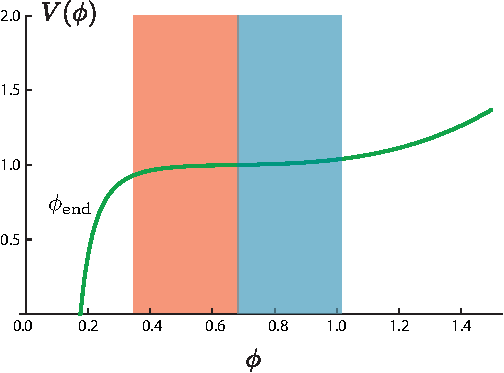
\includegraphics[width=.55\textwidth]{Fractional}
%\vspace{-0.5cm}
\caption{変曲点インフレーション．}
\label{fig:fractional}
\end{figure}



\end{enumerate}


\subsubsection{まとめと展望}
\label{sec:perspective}

\S\ref{sec:eft}では，eta問題が次元6のプランク・スケールで抑制された演算子にどのように敏感であるかを説明した．
インフレーションの有効場理論模型では，寄与する補正項の相殺によるeta問題の解決を，もちろん常に{\it 仮定}できる．言い換えれば，次元6のプランク・スケールで抑制された補正の間で近似的な相殺が起こり，平坦なポテンシャル $V(\phi)$ が生じると仮定できる．
弦理論のインフレーション模型でこの道を選ぶことは，プランク・スケールで抑制された寄与を，弦理論をのぞく（限られた）窓として用いる機会を放棄することである．さらに，いったん $\phi$ を弦コンパクト化の物理的自由度と同定すれば，ポテンシャルの正確な形は原理的にはコンパクト化の残りのデータによって完全に指定される．（この段階で解析に推測を混ぜ込むと，実質的に「弦理論から導出された」シナリオが「弦理論に着想を得た」シナリオに変わってしまう．後者は宇宙論的模型としては興味深くても，弦理論の理解には寄与しない．）
したがって，eta問題の克服は詳細な計算の問題となる．原理的には完全な
ポテンシャルを第一原理から計算でき，実際にも多くの場合， %at least
最低次のポテンシャルへの補正を分類できる．

本節では，ワープしたDブレーン・インフレーションの主要な補正を列挙し，偶然の相殺（または微調整）によって，限られたインフラトンの値の範囲でetaを小さくできることを示した．
これは，D3ブレーンをもつワープしたスロート模型にインフレーション解が存在することの非自明な証明を与える．


\subsectionlink{{\sl 事例研究：}アクシオン・モノドロミー・インフレーション}
\label{sec:LargeField} 

次に，第2の事例研究として，弦理論における大場インフレーションの例に移る．
\S\ref{sec:EFT}で論じたように，これらの模型の特有の課題は，プランク・スケールに近い質量をもつ自由度とインフラトンとの結合から生じる，インフラトン・ポテンシャルへの寄与の無限級数を制御しなければならないことである．これらの項を直接列挙して微調整すること（\S\ref{sec:warped}の小場の例で行ったこと）は明らかに非現実的であり，これらの項を制御または禁止する対称性の議論を構築することが不可欠と思われる．

この方向で影響力のある提案が自然インフレーション~\cite{Freese:1990rb}（{\bf 第1講}参照）であり，そこでは擬南部--ゴールドストーン粒子（すなわちアクシオン）がインフラトンである．摂動論的には，アクシオン場 $a$ は連続シフト対称性 $a\to a+const $ をもつが，これは非摂動効果によって離散対称性 $a\to a+2\pi$ へと破れる．
非摂動効果は周期的なポテンシャルを生成する：
\begin{equation}
V(\phi)=\frac{\Lambda^4}{2} \left[ 1- \cos \left({\phi \over f}\right) \right]+ \ldots\, ,
\end{equation}
ここで $\Lambda$ は力学的に生成されるスケール，$f$ はアクシオン崩壊定数と呼ばれる量であり，$\phi \equiv  a f$ である．省略した項は高調波である．
%The reader can easily verify from Eq.~(\ref{equ:SR}) that if the omitted terms are negligible and $f>M_{\rm pl}$, this potential can drive prolonged inflation.

上で説明したように，シフト対称性によって超プランク的な場の変位範囲が保護される有効理論を提案する際には，その構造に紫外完備化が存在するかが重要な問題となる．したがって，弦理論において崩壊定数 $f>M_{\rm pl}$ をもつアクシオンを探すべきである．


\subsubsection{弦理論におけるアクシオン}

\subsubsection*{$p$形式から生じるアクシオン}

弦コンパクト化には多くのアクシオンが存在し，コンパクト空間の $p$サイクル上で $p$形式ゲージ・ポテンシャルを積分することによって生じる．例えばIIB型弦理論では，Neveu--Schwarz（NS）2形式 $B$ を2サイクル $\Sigma_i$ 上で積分して得られるアクシオン $b_i =2\pi \int_{\Sigma_i} B$ と，Ramond--Ramond（RR）2形式 $C$ から得られるアクシオン $c_i =2\pi \int_{\Sigma_i} C$ がある．
フラックスや，巻き付いて時空を満たすブレーンのような追加要素がなければ，これらのアクシオンのポテンシャルは古典的に平坦であり，10次元作用のゲージ不変性に由来する連続シフト対称性をもつ．インスタントン効果はこの対称性を離散部分群 $b_i \to b_i + 2\pi$（$c_i \to c_i + 2\pi$）へと破る．
これによってアクシオン・ポテンシャルに周期的な寄与が生じる．その周期をこれから見積もる．
弦理論の既知の計算可能な極限では，アクシオン崩壊定数は $M_{\rm pl}$ より小さいことがわかる~\cite{Banks:2003sx,Svrcek:2006yi}．弦コンパクト化にあまり馴染みのない読者は，この主張を受け入れて\S\ref{sec:axioninflation}に進んでも，話の流れを追ううえで支障はない．

\begin{figure}[h!]
	\centering
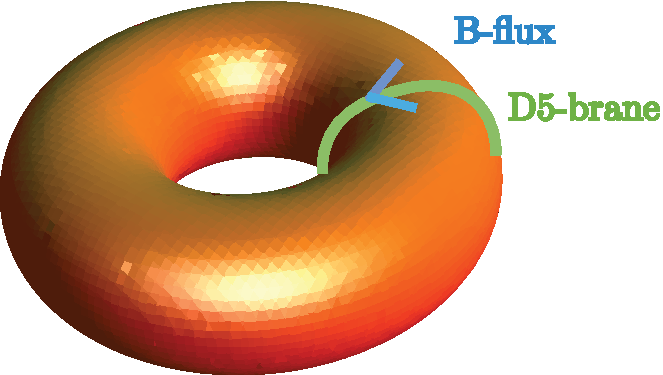
\includegraphics[width=.55\textwidth]{torus}
%\vspace{-0.5cm}
\caption{アクシオン・モノドロミー}
\label{fig:torus}
\end{figure}

\subsubsection*{弦理論におけるアクシオン崩壊定数}

コンパクト空間 $X$ 上の2形式の空間 $H^2(X, Z)$ の基底を $\omega^i$ とし，$\int_{\Sigma_i} \omega^j = \alpha'\delta_{i}^{~j}$ とする．
NS 2形式ポテンシャル $B$ は次のように展開できる：
\begin{equation}
B= \frac{1}{2\pi} \sum_i b_{i}(x)\, \omega^i\, ,
\end{equation}
ここで $x$ は4次元時空の座標である．
アクシオン崩壊定数は，その運動項の規格化から読み取れる．この場合，運動項は10次元の次の項から降りてくる：
\beq
\frac{1}{(2\pi)^7 g_s^2\alpha'^4}\int  \d^{10}x \ {1\over 2} |\d B|^2\quad \supset
\quad \frac{1}{2} \int \d^4 x \sqrt{-g}\, \gamma^{ij} (\partial^{\mu}b_i\partial_{\mu} b_j)\,
 \, ,
\eeq
ここで
\beq
\label{equ:gamma}
\gamma^{ij} \equiv \frac{1}{6 (2\pi)^9 g_s^2 \alpha'^4} \int_X \omega^i \wedge \star_6\, \omega^j\,
\eeq
であり，$\star_6$ は6次元のホッジ星演算子である．
内部空間 $X$ 上の積分を行い，場の空間の計量を $\gamma^{ij} \to f_i^2 \delta_{ij}$ と対角化することで，アクシオン崩壊定数 $f_i$ を取り出せる．

普遍的な結論を導くのは時期尚早だが，蓄積された証拠は，弦理論の計算可能な極限では得られるアクシオンの周期が常に $M_{\rm pl}$ より小さいことを示唆している~\cite{Banks:2003sx,Svrcek:2006yi}．
これは議論に不可欠なので，簡単な例で示そう．コンパクト化が等方的で，典型的な長さスケールが $L$，体積が $L^6$ であると仮定する．このとき
\beq \alpha' M_{\rm pl}^{2}= \frac{2}{(2\pi)^7}\frac{L^6}{g_s^2\alpha'^3} \eeq
を用いると，式~(\ref{equ:gamma}) から
\begin{equation}
f^2\approx M_{\rm pl}^2\, \frac{\alpha'^2}{6(2\pi)^2 L^4}\, .
\end{equation}
制御可能なコンパクト化では $L \gg \sqrt{\alpha'}$ が必要なので，$f \ll M_{\rm pl}$ となる．
はるかに一般的な配置でも，定性的に同様の結論が成り立つ~\cite{Banks:2003sx,Svrcek:2006yi}．

\subsubsection{弦理論におけるアクシオン・インフレーション}
\label{sec:axioninflation}

上の結果は，単一のアクシオン場による自然インフレーションが，既知の弦コンパクト化では実現できないことを意味するように見える．弦理論は多くのアクシオンを与えるが，十分に広い場の変位範囲をもつものは一つもない．しかし，この障害を回避するための妥当な提案が少なくとも二つある．

\subsubsection*{Nフレーション}

最初の提案は，数百個ものアクシオンの集団励起が，インフレーションに十分な有効な場の変位範囲をもちうるというものであった~\cite{Nflation, Easther:2005zr}．
インフラトンの役割は，集団場
\beq
\phi^2 = \sum_{i=1}^N \phi_i^2\, .
\eeq
個々の場の変位範囲がプランク・スケール未満，$\phi_i < M_{\rm pl}$ であっても，場の数 $N$ が十分に大きければ，有効場 $\phi$ は超プランク的な変位をもちうる．
この「Nフレーション」の提案は補助インフレーション~\cite{Liddle:1998jc}の具体例だが，特に重要なのは，インフレーションを妨げる補正からアクシオン・ポテンシャルを保護するうえで，対称性が役立つことである．有望ではあるものの，このシナリオの原理実証はまだなされていない．多数の軽い場が存在すると，ニュートン定数に問題となる繰り込みが生じ，その結果として有効な場の変位範囲が狭くなるためである．
Nフレーションの最近の研究については，文献~\cite{Kallosh:2007cc, Grimm:2007hs}参照．


\subsubsection*{アクシオン・モノドロミー}

ここでは代わりに，一つの周期的なアクシオン場が何周もする間インフレーションが続くことを可能にする，基本的な機構である{\it{モノドロミー}}を説明する．（素朴な）配置空間の閉じたループに沿って輸送したとき，系が新しい配置に到達するなら，その系はモノドロミーをもつという．典型例は螺旋階段である．素朴な配置空間は角度座標で記述されるが，$2\pi$ だけ移動すると系は変化する．（実際，この簡単な模型は，アクシオン・モノドロミー・インフレーションのポテンシャルを非常によく記述することがわかる．）
モノドロミーを用いて弦理論で制御可能な大場インフレーションを実現するという考えは，Silverstein と Westphal~\cite{Silverstein:2008sg}によって初めて提案された．彼らは，ニル多様体の内部に巻き付いたD4ブレーンを含む模型を論じた．本節では，その後に提案された文献~\cite{MSW}のアクシオン・モノドロミーに焦点を当てる．この場合，アクシオンによってパラメータ化された場の空間の円に沿って輸送すると，4次元のポテンシャル・エネルギーにモノドロミーが生じる．

このようなモノドロミーはさまざまなコンパクト化で可能だが，ここでは一つの具体例に集中する．カラビ--ヤウ・オリエンティフォールド上のIIB型弦理論を考えよう．これは世界面の向きの反転と幾何学的な対合を含む離散対称性によって，カラビ--ヤウ多様体の商を取ったものである．具体的には，対合は固定点と固定4サイクルをもち，それらはそれぞれO3プレーンとO7プレーンとして知られていると仮定する．さらにコンパクト化が，適切な2サイクル $\Sigma$ に巻き付き時空を満たすD5ブレーンを含むなら，アクシオン $b=2\pi \int_{\Sigma}B$ はポテンシャル・エネルギーにモノドロミーを示しうる．（同様に，巻き付いたNS5ブレーンはアクシオン $c=2\pi \int_{\Sigma}C$ にモノドロミーを生じさせる．）
言い換えれば，$\Sigma$ に巻き付くD5ブレーンのポテンシャル・エネルギーは，アクシオンの周期関数では{\it ない}．巻き付いたブレーンの存在によってアクシオン作用のシフト対称性が破れるからである．実際，$b$ の増加とともにポテンシャル・エネルギーは際限なく増大する．

D5ブレーンの場合，問題のポテンシャルは，巻き付いたDブレーンのDirac--Born--Infeld作用から生じる：
\begin{eqnarray}
S_{\rm DBI} &=& \frac{1}{(2\pi)^5 g_s \alpha'^3} \int_{{\cal M}_4 \times \Sigma}  \d^6 \xi \, \sqrt{\det(G+B)} \\
&=& \frac{1}{(2\pi)^6 g_s \alpha'^2} \int_{{\cal M}_4} \hskip -6pt \d^4 x\, \sqrt{-g} \, \sqrt{(2\pi)^2\ell_\Sigma^4 + b^2} \label{equ:bb}\, ,
\end{eqnarray}
ここで $\ell_\Sigma$ は弦単位で測った2サイクル $\Sigma$ の大きさである．
式~(\ref{equ:bb}) のブレーン・エネルギーは，シフト対称性 $b\to b +2\pi$ のもとで明らかに不変ではない．ただし，この対称性は，巻き付いたD5ブレーンを取り除いた対応するコンパクト化の対称性である．このように，DBI作用は $b$ のモノドロミーを直接もたらす．さらに，$b \gg \ell_\Sigma^2$ では，ポテンシャルは正準的に規格化された場 $\varphi_b \propto b$ に対して漸近的に{\it{線形}}となる．

\vskip 6pt
この模型のインフレーションのダイナミクスは，定性的には次のとおりである．まず，曲線 $\Sigma$ に巻き付いたD5ブレーンを考え，その上の $ \int_\Sigma B$ を大きく取る．言い換えれば，アクシオン $b$ は大きな初期真空期待値をもつ．この真空期待値が減少するにつれてインフレーションが進み，最終的には $\int_\Sigma B = 0$ となり，D5ブレーンはほぼ「空」，すなわち世界体積上のフラックスがほとんどない状態となる．この過程でD5ブレーンは動かず，閉弦モジュライもほとんど変化しない．アクシオンの真空期待値が小さくなると，上で述べた漸近的に線形なポテンシャルの近似は不正確になり，ポテンシャルの曲率が無視できなくなる．式~(\ref{equ:bb}) 参照．
この段階で，アクシオンは原点のまわりに振動し始める．アクシオンと，閉弦モードまたは開弦モードであるほかの自由度との結合が，インフラトン振動からエネルギーを奪う．このエネルギーの十分な割合が最終的に可視セクターの自由度へ伝われば，高温ビッグバンが始まる．可視セクターは，例えばコンパクト化の別の場所にあるDブレーンの重なりの上に存在しうる．再加熱の詳細は標準模型の自由度とインフラトンの結合の形に強く依存しており，これはこの模型だけでなく，より一般の弦インフレーションにおいても重要な未解決問題である．
% (For representative work on reheating after string inflation, see \cite{reheating}.)


\subsubsection{コンパクト化についての考察}

アクシオン・モノドロミー・インフレーションの基本的な考えを説明したが，提案したインフレーション機構がモジュライ安定化と両立し，整合的なコンパクト化で実現できることを，なお保証しなければならない．直ちに懸念されるのは，上で特定した線形項以外にも，インフレーション中に重要な影響を及ぼすポテンシャルへの追加寄与があるかどうかである．本総説を通じて強調してきたように，インフラトン・ポテンシャルを保護する対称性がなければ，モジュライ安定化による一般的な補正が $\Delta\eta\sim {\cal O}(1)$ の寄与を与えると予想される．
したがって，インフラトン・ポテンシャルを保護する連続シフト対称性が，安定化されたコンパクト化でも適切な程度に保たれることを確認するのが不可欠である．
非摂動効果が役割を果たす特別なモジュライ安定化の場合には，シフト対称性が損なわれないことを保証するのは非常に微妙な問題となりうる．
これは文献~\cite{MSW}で詳しく説明されている．



\subsubsection{まとめと展望}
\label{sec:axionS}

Lyth限界は，観測可能な重力波信号が，インフレーション中にインフラトン場が超プランク的な距離を移動することと結びついていることを示す．
このため，大場インフレーションの有効場理論模型では，超プランク的な範囲にわたりポテンシャルの平坦性を保護するシフト対称性が必要となる．
したがって，そのようなシフト対称性が弦理論で生じ，大場インフレーションの実現に利用できるかどうかが，重要な問題となっている．

本節では，超プランク的な範囲にわたってポテンシャルを保護する，弦理論におけるシフト対称性の最初の例が得られ始めていると論じた．
モノドロミーの二重の役割を説明した．i）小さな基本領域を繰り返し通過できるようにすることで，大きな運動学的な場の範囲 $\Delta \phi > M_{\rm pl}$ を生む．ii）シフト対称性と組み合わさることで，超プランク的な範囲にわたるポテンシャルの補正を制御する．
%LM
$V$ によってごく弱くしか破れないシフト対称性は，一つの基本領域内の補正 $\Delta V$ を制御し，
%the monodromy 
さらに，ある基本領域の補正をほかのあらゆる基本領域の補正と関係づける．
したがってモノドロミーは，大場の問題を実質的に小場の問題へ還元する~\cite{Silverstein:2008sg}．

これらの模型と，それらが生じるコンパクト化を理解するにはさらに研究が必要だが，モノドロミーは弦理論において大場インフレーション，したがって観測可能な重力波信号を実現する，頑健でかなり有望な機構と思われる．



\sectionlink{今後の展望}

\subsectionlink{理論面の展望}

本講で示せたことを願うが，近年の理論的進歩は目覚ましい．10年前には弦理論と宇宙論を結びつける提案はわずかしかなく，モジュライを安定化する問題にもまだ取り組まれていなかった．現在では弦理論を動機とする多様なインフレーション模型があり，そのうち最もよく研究された例には，モジュライ安定化についての情報が組み込まれている．さらに，弦理論におけるいくつかのインフレーション機構は，関連するすべての補正を含めてモジュライを完全に安定化しても存続するという意味で，頑健であることが示されている．

弦理論でインフレーションが可能であることを示した以外に，何が達成されたのだろうか．われわれの見方では，弦理論における明示的なインフレーション模型の主な用途は，インフレーションの量子重力に対する感度を調べる検証例，または玩具模型としての役割にある．理論面では，これらの模型は一般の場の理論におけるインフレーションの実現でeta問題が重要であることを強調し，場の理論では不自然に見えても弦理論では自然と思われるインフレーション機構を導き，原始テンソルモードの検出がもつ意味についての理解を明確にしてきた．

今後の理論的進歩の方向を予測するのはもちろん難しい．特に，弦理論における予見できない根本的な進歩によって，インフレーション模型構築に使える道具が増えることが期待されるからである．
しかし，モジュライ安定化がさらに着実に進歩し，すべてのモジュライが安定化された明示的な例が追加されると予想してよいだろう．そのようなコンパクト化における完全に明示的なインフレーション模型も，間違いなく続いて現れるはずである．
現在，M理論やヘテロティック弦理論で成功した模型は少なく，穏やかな仮定のもとで，ある種のIIA型コンパクト化ではインフレーションが不可能であることが示せる~\cite{Hertzberg:2007wc, Flauger:2008ad, Caviezel:2008tf}．弦理論の一つの弱結合極限で，ほかの極限よりもインフレーションがはるかに自然だということになれば意外である．現状の差は，各極限で現在利用できるモジュライ安定化の道具の違いにも一部起因すると考えられる．より多様な弦真空でインフレーションがどのように生じうるかを理解することは，明らかに有用であろう．

弦理論で現在得られているインフレーション模型は，整合性条件（例えばタドポール相殺）と，ある程度の計算可能性の必要性から生じる，厳しい理論的制約を受ける．これらの制約は，宇宙論的観測量の間の相関，すなわち予測をもたらす．より一般的な弦コンパクト化を調べられるようになるにつれ，これらの制約の一部は間違いなく消えるだろう．しかし一部は残り，弦理論から導かれるインフレーションの有効作用の集合が，一般の場の量子論におけるインフレーションの有効作用の集合の真部分集合になることを期待できる．このような主張を確立するには，現在よりもはるかに包括的な弦コンパクト化の理解が必要であろう．



\subsectionlink{観測的な痕跡はあるか？}
\label{sec:obs}

本講で述べたインフレーションの理論的側面が興味深い大きな理由は，現在および将来の宇宙論データを用いて，実験的に{\it 検証}できることである（{\bf 第3講}参照）．

%In order to describe this connection, we will very briefly review recent achievements and near-future prospects in observational cosmology.


本講義を通じて繰り返し強調したように，インフレーションを最も劇的に確認するのは $B$モード偏光の検出であろう．それによってインフレーションのエネルギー・スケールが確立され，インフラトンが超プランク的な距離を移動したことが示される．
本講で論じたように，超プランク的な変位は，インフラトンの有効作用がプランク・スケールの物理に特に敏感となる重要な場合である．テンソル摂動が模型を判別する力の具体例として，原始重力波が検出されれば，\S\ref{sec:warped}のワープしたD3ブレーン・インフレーション・シナリオは排除される~\cite{Baumann:2006cd}．一方，上限 $r<0.07$（または $r\gg 0.07$ での検出）は，\S\ref{sec:LargeField}のアクシオン・モノドロミー・シナリオを排除する~\cite{MSW}．

さらに，単一場のスローロール・インフレーションは，多くの宇宙論的観測量について信号がないという予測をするため，別の機会も生じる．原始スカラー揺らぎは，高い精度でスケール不変，ガウス的，断熱的であると予測されるからである．したがって，非ガウス性，等曲率揺らぎ，または大きなスケール依存性（ランニング）の検出は，単一場のスローロール・インフレーションを排除する．大きな非ガウス性，非断熱性，またはスケール依存性を許すインフレーションの有効作用には，高階微分相互作用や複数の軽い場が必要となることが多く，そのような作用は弦理論ではかなり自然に生じる．本講では，インフラトン・ポテンシャルのプランク・スケールの物理に対する感度に焦点を当てたが，インフラトンの運動項も同様に紫外物理に敏感であり，弦理論は大きな非ガウス性を生みうる高階微分相互作用を理解するための有望な枠組みを与える~\cite{DBI,Alishahiha:2004eh}．

最後に，残存する宇宙ひもやほかの位相欠陥によって誘起されるCMBの温度・偏光異方性は，インフレーションの終わりまたはその後の時代の物理を探る手段となる．
宇宙ひもはブレーン・反ブレーン・インフレーションの終わりに自動的に生成され~\cite{Sarangi, CMP}，その結果生じる宇宙ひもネットワークの安定性と現象論的性質は，ワープ幾何の性質によって決まる．重力レンズ効果や特徴的な重力波バーストを通じた宇宙超ひもの検出は，胸の躍る展望である．\\

%\subsectionlink{Conclusions}


%The theoretical community will eagerly await the coming generation of experimental results \cite{Baumann:2008aq}, in the hope of extracting further clues about the physical properties of the early universe.





\newpage
\sectionlink{{\sl まとめ}：第5講}

\begingroup
\setlength{\abovedisplayskip}{5pt}
\setlength{\belowdisplayskip}{5pt}
\setlength{\abovedisplayshortskip}{3pt}
\setlength{\belowdisplayshortskip}{3pt}
近年の多くの著者による研究を通じて，弦理論における頑健なインフレーション機構が現れてきた（最近の総説については文献~\cite{BMReview, Burgess:2007pz, Kallosh:2007ig, Linde:2005dd, McAllister:2007bg, Cline:2006hu}参照）．これらの研究の主な動機は，インフレーションの有効作用が重力の紫外完備化に敏感であることと，高精度の宇宙論データを用いた実証的な検証の見通しである．

本講では，二つの例を通じて{\it インフレーションの紫外物理に対する感度}を示した：

\begin{itemize}
\item {\it eta問題}

etaパラメータ（またはインフラトン質量）の小ささは，次元6のプランク・スケールで抑制された補正に敏感である：
\beq
\Delta V \sim V \frac{\phi^2}{\Mp^2} \qquad \Rightarrow \qquad \Delta \eta_{\rm v} \sim 1\, . \nonumber
\eeq

このような項は，低エネルギー有効理論を得るために（カットオフより上の）重い自由度を積分消去すると生じる．
ワープしたブレーン・インフレーションを例として，この問題が弦理論の計算でどのように明示されるかを示した~\cite{Baumann:2006th, Baumann:2007ah, Baumann:2008kq, BaumannProgress}．

\item {\it 大場模型におけるテンソルモード}

インフレーションが観測可能な振幅の重力波を生成するには，インフラトン場が超プランク的な距離を移動する必要がある．
超プランク的な範囲にわたりインフレーション・ポテンシャルの平坦性を保護することは難しい：
\begin{itemize}
\item {\it シフト対称性がない場合}

特別な対称性がない場合，大場インフレーションのポテンシャルは，プランク・スケールで抑制された演算子の無限級数に敏感になる：
\beq
{\cal L}_{\rm eff}(\phi) = -\frac{1}{2}(\partial \phi)^2 - \frac{1}{2} m^2 \phi^2 - \frac{1}{4} \lambda \phi^4 - \sum_{p=1}^\infty \left[ \lambda_p \phi^4  + \nu_p (\partial \phi)^2    \right] \left( \frac{\phi}{M_{\rm pl}} \right)^{2p}+ \cdots \ . \nonumber
\eeq
この場合，超プランク的な範囲にわたるポテンシャルの平坦性には，多数の展開パラメータ $\lambda_p$ の微調整が必要となる（一つの質量パラメータの調整だけを必要とするeta問題と比較されたい）．

\item {\it シフト対称性がある場合}

インフラトン場がシフト対称性 $\phi \to \phi + const.$ を満たすなら，小さな係数 $\lambda_p$ をもつカオス的インフレーションの作用
 \beq
 {\cal L}_{\rm eff}(\phi) =- \frac{1}{2} (\partial \phi)^2 - \lambda_p\, \phi^p\, , \nonumber
 \eeq
は「技術的に自然」である．
\end{itemize}
したがって，検出可能な重力波を伴うインフレーション模型を構築するには，大きな運動学的範囲 $\Delta \phi > \Mp$ と，完全な弦理論で近似的に保たれるシフト対称性に保護されたポテンシャルの両方をもつ配置を，弦理論の中で見いだすことが目標となる．
このような模型は最近，文献~\cite{Silverstein:2008sg, MSW, Flauger:2009ab}で構築された．
\end{itemize}




%\newpage
%\sectionlink{{\sl Problem Set}: Lecture 4}


\endgroup
\newpage
\part{結論}


\sectionlink{{\sl 振り返り}：インフレーションに関するTASI講義}

%I showed different versions of Fig.~\ref{fig:summary} at the beginning of each of my lectures at {\sl TASI 2009}.

図~\ref{fig:summary}は，本講義で説明した重要な概念の多くをまとめている．

\begin{figure}[h!]
    \centering
        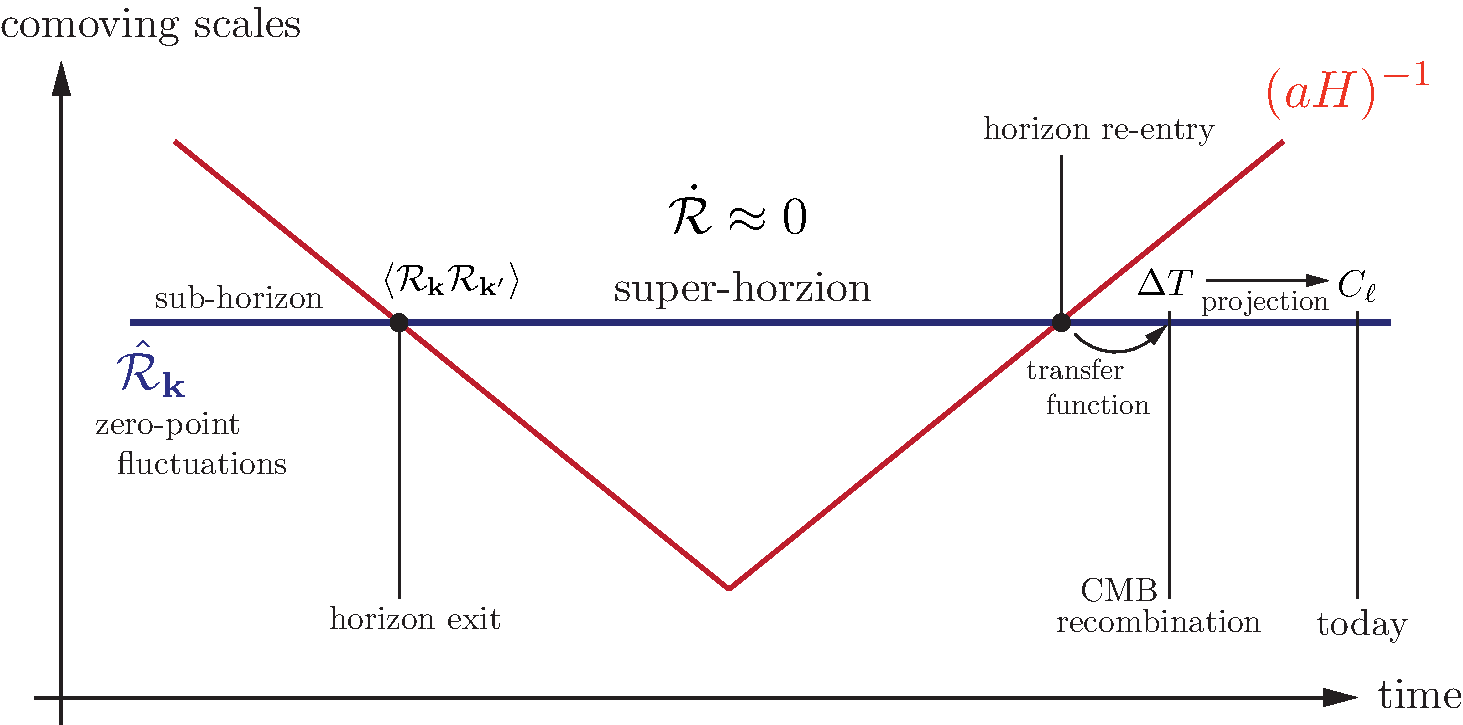
\includegraphics[width=0.9\textwidth]{summary}
    \caption{\small インフレーション宇宙における地平線の発展と摂動の生成．} % (see Figures \ref{fig:WMAP2} and \ref{fig:CMBparam}).}
    \label{fig:summary}
\end{figure} 


\begin{itemize}
\item {\bf 第1講}：インフレーションを，共動ハッブル半径 $(a H)^{-1}$ が減少する極初期宇宙の時期と定義した．この重要な特徴が地平線問題と平坦性問題の解決の核心であることを説明した．再結合時の地平線を超えるスケールで見られるCMB揺らぎの，一見すると因果性に反する相関は，それらのスケールがインフレーション中には地平線内にあり，したがって因果的につながっていたことで説明される．
\item {\bf 第2講}：モードはインフレーション中に地平線を出て，後の通常のFRW膨張期に再び地平線に入る．インフレーション中のスカラー揺らぎを，共動曲率摂動 ${\cal R}$ で記述した．${\cal R}$ の決定的な特徴は，地平線を超えるスケールで凍結し，$\dot \R \approx 0$ となることである．したがって，${\cal R}$ の初期条件はインフレーション中の地平線脱出時に計算でき，そのまま地平線への再突入時まで引き継がれる（かなり弱い仮定のもとで，これは未知の再加熱の物理に依存しない）．第2講では，地平線脱出時の曲率摂動のパワースペクトル $\langle {\cal R}_{\bf k} {\cal R}_{\bf k'} \rangle = (2\pi)^3 \delta({\bf k}+{\bf k'}) P_\R(k)$ を計算した．
\item {\bf 第3講}：地平線への再突入後，曲率摂動 ${\cal R}$ は再結合時のCMB温度の揺らぎ $\Delta T$ へと発展する．この地平線内での発展は，第3講で論じた伝達関数によって記述される．そして今日，われわれが見るのは，最終散乱面からわれわれへと投影されたCMB揺らぎである．
実験はCMB温度揺らぎの角度パワースペクトル $C_\ell$ を測定する．第3講では，観測されたCMB異方性の角度パワースペクトルを，インフレーション中に生成された原始曲率揺らぎのパワースペクトル $P_\R(k)$ に関係づける方法を説明した．
したがって，地平線内での発展を逆にたどり，投影効果を取り除くことで，CMB観測はインフレーションの摂動を探る強力な手段となる．
\item {\bf 第4講}：原始曲率摂動の3点関数 $\langle {\cal R}_{{\bf k}_1} {\cal R}_{{\bf k}_2} \R_{{\bf k}_3} \rangle = (2\pi)^3 \delta({\bf k}_1+{\bf k}_2 + {\bf k}_3) B_\R(k_1, k_2, k_3)$ は，原始揺らぎが十分に非ガウス的であれば，インフレーションの物理を探る追加の手段となる．
\end{itemize}

\sectionlink{将来の展望と未解決問題}
\label{sec:conclusion}

インフレーションに対する現在の観測的証拠を述べ，その物理をさらに検証するための将来の観測機会を取り上げた．
インフレーションを最も直接的に探る二つの手段は，原始テンソルモードと原始非ガウス性である：
\begin{itemize}
\item {\bf Bモード}

原始 $B$モード（インフレーションのテンソルモードがCMB偏光に残す痕跡）の検出は，インフレーションを確認するために可能な観測の中で，明らかに最も特徴的なものである．これによってインフレーションのエネルギー・スケールを測定し，インフラトン場が超プランク的な距離を移動したことを知ることができる．
欧州の{\sl Planck}衛星~\cite{:2006uk}，多くの地上実験や気球実験~\cite{CMBPolWorkshop, Kosowsky:2004sw, Ruhl:2004kv, Taylor:2006jw, Samtleben:2008rb, Yoon:2006jc, Oxley:2005dg, MacTavish:2007kh}，そして計画中の{\sl CMBPol}ミッション~\cite{WhitePaper, Bock:2009xw}は，いずれもインフレーション期からのこの信号の検出を目指している．理論研究者たちは，これらの実験結果を大きな期待とともに待っている．

\item {\bf 非ガウス性}

インフレーションの物理の，やや模型依存性が高い痕跡は，原始揺らぎに非ガウス性が存在する可能性である．単一場のスローロール模型では小さいと予測されるが，複数の場，高階微分相互作用，または非自明な真空状態をもつ模型は，非ガウス的な痕跡を残しうる．フーリエ空間の信号の運動量依存性は，原始揺らぎを生み出した機構を診断する強力な手段である．{\sl Planck}衛星は，原始非ガウス性を高感度で探ることになる．
\end{itemize}

本講義では，インフレーションについてかなり楽観的な見方を提示した．
これは，インフレーションの物理を理解し制約するうえで近年達成された理論・観測両面の大きな進歩を示す一方，この理論がなお直面する重要な概念的問題を省いている．ここでは，これらの理論的課題のいくつかを挙げ，詳細について関連文献を示す：
\begin{itemize}
\item {\bf 初期条件}

本講義では，インフレーションを開始するために必要な初期条件について，ごく表面的にしか触れていない．これは一部には，インフレーションの初期条件があまりよく理解されていないという事情を反映している．

単純なスローロールによるインフレーションの解析では，インフラトンの初期速度は小さく，インフラトン場の初期の非一様性はインフレーションを妨げるほど大きくないと{\it 仮定}した：

\begin{itemize}
\item {\it オーバーシュート問題}

インフレーションが起こるはずのポテンシャル領域の近くで，インフラトンの初期速度が無視できなければ，場は加速膨張を生み出すことなく，その領域を{\it 通り越してしまう}可能性がある．
この問題は小場模型でより深刻になる．そこではしばしば，場が注目する領域に到達する前にハッブル摩擦で十分に減速できないためである．

\begin{figure}[h!]
    \centering
        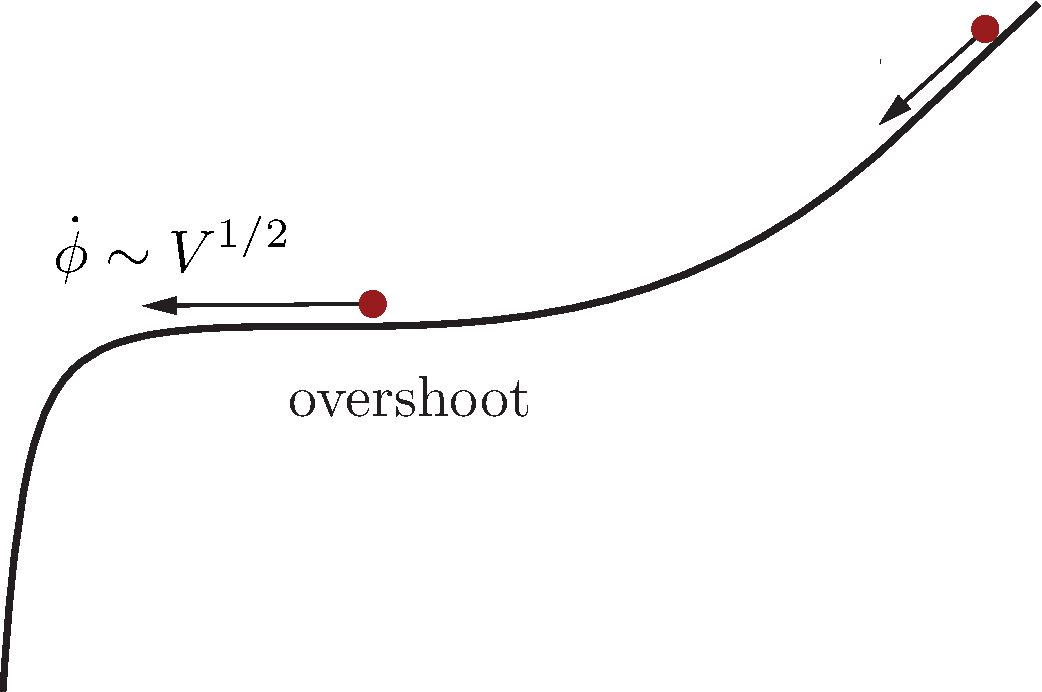
\includegraphics[width=0.38\textwidth]{overshoot}
    \caption{\small オーバーシュート問題の模式図．} % (see Figures \ref{fig:WMAP2} and \ref{fig:CMBparam}).}
    \label{fig:overshoot}
\end{figure} 



\item {\it パッチ問題}

インフラトン場の初期の非一様性は，やはり加速膨張を妨げる勾配エネルギーを与える．
具体例に対する数値解析は，インフレーションを開始するために，通常インフラトン場がその時点の地平線サイズの数倍にわたって滑らかでなければならないことを示している．

\begin{figure}[h!]
    \centering
        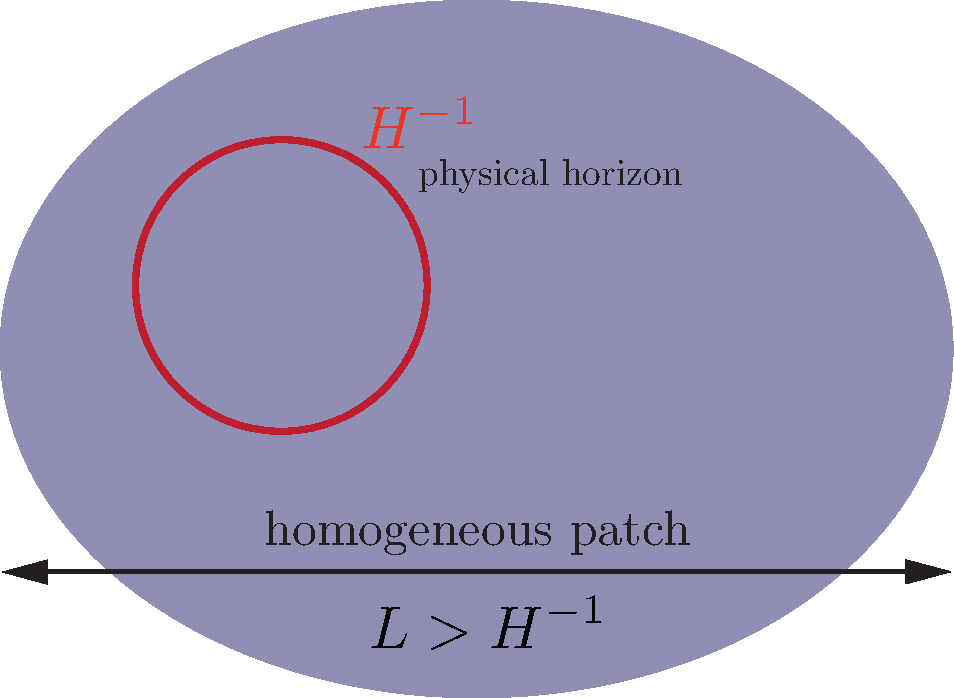
\includegraphics[width=0.38\textwidth]{patch}
    \caption{\small パッチ問題の模式図．} % (see Figures \ref{fig:WMAP2} and \ref{fig:CMBparam}).}
    \label{fig:patch}
\end{figure} 

\end{itemize}

インフレーションに必要な初期条件の微調整が実際にどれほど深刻かは，いまだ十分に理解されていない永遠のインフレーションと測度問題から切り離して論じることはできない．

\item {\bf 永遠のインフレーションと測度問題}

現代的なインフレーションの見方では，大域的にはインフレーションは決して終わらない！
インフレーションは局所的には終わり，FRW宇宙の小領域を作るが，量子揺らぎによって場が高いポテンシャル・エネルギーに保たれる領域が常に存在する．
これらの領域は指数関数的に膨張し続け，インフレーションしている領域の体積をさらに増やす．

インフレーションの初期条件がどれほど起こりやすいか，さらにはインフレーション自体が何を予測するかも，宇宙（または多宇宙）におけるインフレーションする領域としない領域の相対確率に依存する．これが測度問題である．
異なる確率測度を採用すると，インフレーションの初期条件の確率や，特定の観測的特徴（平坦性，スケール不変な揺らぎなど）をもつFRW宇宙の生じやすさが大きく変わりうる．

永遠のインフレーションと測度問題についての詳細は，文献~\cite{Vilenkin:1983xq, Linde:1986fd, Linde:1993nz, Linde:1993xx, GarciaBellido:1993wn,Vilenkin:1994ua, Garriga:2005av, Bousso:2006ev, Linde:2007nm, Bousso:2008hz, DeSimone:2008if, Garriga:2008ks, Winitzki:2008jp, Linde:2008xf}を参照されたい．

\end{itemize}

これらの問題は，インフレーションと宇宙論的初期条件に関する理論的理解を深める余地が，まだ残されていることを示している．
同時に，CMB偏光と小スケールの温度揺らぎの高精度測定の到来は，インフレーション仮説の実際の実験的検証を約束している．


\sectionlink{さらに学ぶための文献案内}

以下の教科書，総説，論文は，本講義の準備に役立ったものである．
学生諸君は，これらの文献からインフレーションについての有益な詳細をさらに学べるだろう．


\subsubsection*{教科書}

\begin{itemize}
\item Mukhanov, {\it 宇宙論の物理的基礎}

初期宇宙論と宇宙論的摂動の理論についての優れた解説．

\item Dodelson, {\it 現代宇宙論}

宇宙マイクロ波背景放射に重点を置いた，宇宙論の優れた本．非常に読みやすく，つまり寝転びながらでも読める．


\item Weinberg, {\it 宇宙論}

Steven Weinbergによる本である！

\item Liddle and Lyth, {\it 宇宙論的インフレーションと大規模構造}

インフレーション宇宙論についての包括的な概説．

\item Longair, {\it 銀河形成}

より天体物理学的な視点から見た宇宙論．

\item Birrell and Davies, {\it 曲がった時空における場の量子論}

曲がった時空における場の量子論の古典的な解説．


\end{itemize}


\subsubsection*{総説}

\begin{itemize}
\item Baumannら, {\it CMB偏光でインフレーションを探る}

CMBPolミッション概念検討のインフレーション作業部会による白書．
60人以上のインフレーションの専門家が協力して，この非常に包括的な総説を執筆した．

\item Baumann and Peiris, {\it 宇宙論的インフレーション：理論と観測}

この総説では，Hiranya Peirisと私が，専門外の読者向けにインフレーションとCMB観測の基礎をまとめた．本講義の読者には初歩的すぎるかもしれないが，就寝前の読み物を探している読者には興味深いかもしれない．

\item Baumann and McAllister, {\it 弦インフレーションの進展}

この総説では，Liam McAllisterと私が，弦理論においてインフレーションを実現するという課題を説明している．

\item Lyth and Riotto, {\it インフレーションの素粒子物理模型}

本講義で不足しているインフレーション模型の構築に関する内容は，ここで見つかる．

\item Bassettら, {\it インフレーションのダイナミクスと再加熱}

本講義で不足している再加熱に関する内容は，ここで見つかる．

\item Kinney, {\it インフレーションに関するTASI講義}

Will Kinneyによる{\sl TASI 2008}の講義は，インフレーションについて最初に読むものとして最適である．
この{\sl TASI 2009}の講義が，2番目の読み物としてよいものになっていれば幸いである．
より技術的な詳細を示すことで，Willの講義を補うよう努めた．

\item Malik and Wands, {\it 宇宙論的摂動}

1次および2次の摂動論についての優れた総説．有用な公式が多数掲載されている．


\item Komatsu, {\it 宇宙マイクロ波背景放射における非ガウス揺らぎの探究}

Eiichiro Komatsuの博士論文には，インフレーションに由来する非ガウス揺らぎについての有用な概説が含まれている．
\end{itemize}



\subsubsection*{原著論文}

インフレーションに関する原著論文の中には非常に読みやすく，一読に値するものがある：

\begin{itemize}
\item Guth, {\it インフレーション宇宙：地平線問題と平坦性問題の解となる可能性}

{\small この古典的論文はもちろん必読である．ビッグバンの謎を非常に明快に説明している．}

\item Maldacena, {\it 単一場のインフレーション模型における原始揺らぎの非ガウス的特徴}

{\small この論文は，スローロール・インフレーションの3点関数を初めて厳密に計算した．また，インフレーションの揺らぎのパワースペクトルの計算について，最も明快かつ洗練された解説の一つを与えている．本講義の扱いは，Maldacenaの論文から大きな影響を受けた．}


{\small }
\end{itemize}

\newpage
